%\documentclass{llncs}
\documentclass[11pt]{article} % use larger type;

\usepackage[utf8]{inputenc} % set input encoding (not needed with XeLaTeX)


%%% PAGE DIMENSIONS
\usepackage{geometry} % to change the page dimensions
\usepackage{graphicx,array}
\usepackage{amsmath}
\usepackage{amssymb}
\usepackage{amsfonts}
\usepackage{epsfig}
\usepackage{float}
%\usepackage{supertabular} % used in B Symbols
\geometry{a4paper} % or letterpaper (US) or a5paper or....

%% Keywords for the B method
\newcommand{\MACHINE}{\operatorname{\mathbf{MACHINE}}}
\newcommand{\REFINEMENT}{\operatorname{\mathbf{REFINEMENT}}}
\newcommand{\IMPLEMENTATION}{\operatorname{\mathbf{IMPLEMENTATION}}}
\newcommand{\REFINES}{\operatorname{\mathbf{REFINES}}}
\newcommand{\SEES}{\operatorname{\mathbf{SEES}}}
\newcommand{\INCLUDES}{\operatorname{\mathbf{INCLUDES}}}
\newcommand{\IMPORTS}{\operatorname{\mathbf{IMPORTS}}}
\newcommand{\SETS}{\operatorname{\mathbf{SETS}}}
\newcommand{\CONSTANTS}{\operatorname{\mathbf{CONSTANTS}}}
\newcommand{\PROPERTIES}{\operatorname{\mathbf{PROPERTIES}}}
\newcommand{\CONCRETE}{\operatorname{\mathbf{CONCRETE}}}
\newcommand{\VARIABLES}{\operatorname{\mathbf{VARIABLES}}}
\newcommand{\ASSERTIONS}{\operatorname{\mathbf{ASSERTIONS}}}
\newcommand{\CONCRETEVARIABLES}{\operatorname{\mathbf{CONCRETE\_VARIABLES}}}
\newcommand{\DEFINITIONS}{\operatorname{\mathbf{DEFINITIONS}}}
\newcommand{\VAR}{\operatorname{\mathbf{VAR}}}
\newcommand{\IN}{\operatorname{\mathbf{IN}}}
\newcommand{\INVARIANT}{\operatorname{\mathbf{INVARIANT}}}
\newcommand{\INITIALISATION}{\operatorname{\mathbf{INITIALISATION}}}
\newcommand{\OPERATIONS}{\operatorname{\mathbf{OPERATIONS}}}
\newcommand{\BEGIN}{\operatorname{\mathbf{BEGIN}}}
\newcommand{\END}{\operatorname{\mathbf{END}}}
\newcommand{\PRE}{\operatorname{\mathbf{PRE}}}
\newcommand{\IF}{\operatorname{\mathbf{IF}}}
\newcommand{\THEN}{\operatorname{\mathbf{THEN}}}
\newcommand{\ELSE}{\operatorname{\mathbf{ELSE}}}
\newcommand{\ELSIF}{\operatorname{\mathbf{ELSIF}}}
\newcommand{\ANY}{\operatorname{\mathbf{ANY}}}
\newcommand{\WHERE}{\operatorname{\mathbf{WHERE}}}
\newcommand{\CASE}{\operatorname{\mathbf{CASE}}}
\newcommand{\OF}{\operatorname{\mathbf{OF}}}
\newcommand{\EITHER}{\operatorname{\mathbf{EITHER}}}
\newcommand{\AND}{\operatorname{\mathbf{AND}}}
\newcommand{\OR}{\operatorname{\mathbf{OR}}}
\newcommand{\NOT}{\operatorname{\mathbf{NOT}}}
\newcommand{\WHILE}{\operatorname{\mathbf{WHILE}}}
\newcommand{\DO}{\operatorname{\mathbf{DO}}}
\newcommand{\VARIANT}{\operatorname{\mathbf{VARIANT}}}
\newcommand{\FALSE}{\operatorname{\mathbf{FALSE}}}
\newcommand{\TRUE}{\operatorname{\mathbf{TRUE}}}

%% Commonly used math entities
\newcommand{\pow}{\operatorname{\mathbb{P}}}
\newcommand{\nat}{\operatorname{\mathbb{N}}}
\newcommand{\pfun}{\operatorname{\rightarrow\mkern-22mu+}}
\newcommand{\fset}{\operatorname{\mathbb{F}}}
\newcommand{\dom}{\operatorname{\mbox{dom}}}
\newcommand{\ran}{\operatorname{\mbox{ran}}}
\newcommand{\natone}{\operatorname{\mathbb{N}_1}}
\newcommand{\integer}{\operatorname{\mathbb{Z}}}
\newcommand{\fun}{\operatorname{\rightarrow}}
\newcommand{\domr}{\operatorname{\triangleleft}}
\newcommand{\seq}{\operatorname{\mathbf{seq1}}}
\newcommand{\ovr}{\operatorname{\oplus}}
\newcommand{\BOOL}{\operatorname{\mathbf{BOOL}}}
\newcommand{\pred}{\operatorname{\mathbf{pred}}}
\newcommand{\Bsucc}{\operatorname{\mathbf{succ}}}


%\usepackage{supertabular}

% DEFINITION DES CARACTERES MATHEMATIQUES B
%------------------------------------------
\def\@setmcodes#1#2#3{{\count0=#1 \count1=#3
	\loop \global\mathcode\count0=\count1 \ifnum \count0<#2
	\advance\count0 by1 \advance\count1 by1 \repeat}}

%\@setmcodes{`A}{`Z}{"7441}
%\@setmcodes{`a}{`z}{"7461}

\mathcode`\;="8000 % Makes ; active in math mode
{\catcode`\;=\active \gdef;{\semicolon\;}}
\mathchardef\semicolon="003B
%    Nominal distance from top of paper to top of page
% \topmargin 0 pt
% \textheight 53\baselineskip
% 
% %   Left margin on odd-numbered pages
% \oddsidemargin  0.15 in
% %   Left margin on even-numbered pages
% \evensidemargin 0.35 in
% %   Width of marginal notes.
% \marginparwidth 1 in
% %   Note that \oddsidemargin = \evensidemargin
% \oddsidemargin 0.25 in
% \evensidemargin 0.25 in
% \marginparwidth 0.75 in
% \textwidth 5.875 in % Width of text line.
% 
% \setlength{\parindent}{0pt}
% \setlength{\parskip}{0ex}

% DEFINITION DES FONTS
%---------------------
% The AMS extra symbol fonts are loaded.
% Note: sometimes called euxm10
\font\msx=msam10
% Note: sometimes called euym10
\font\msy=msbm10

\newfam\msxfam \textfont\msxfam=\msx
\newfam\msyfam \textfont\msyfam=\msy

\def\famletter#1{\ifcase #1 0\or 1\or 2\or 3\or 4\or 5\or 6\or 7\or
	8\or 9\or A\or B\or C\or D\or E\or F\fi}

\edef\fx{\famletter\msxfam}
\edef\fy{\famletter\msyfam}

\def\bbold{\fam\msyfam \msy}

% SYMBOLES B
%-----------
% makes a quoted expression in mathematical text
\def\token#1{\hbox{`$#1$'}}
% used for error messages in Z specs
\def\report#1{\hbox{`{\tt #1}'}}

% \@myop makes an operator, with a strut to defeat TeX's vertical adjustment.
\def\@myop#1{\mathop{\mathstrut{#1}}\nolimits}

% This underscore doesn't have the little kern --- you get an italic
% correction anyway in math mode.
\def\_{\leavevmode \vbox{\hrule width0.5em}}

% Save \q as \xq for quantifiers q.
\let\xforall=\forall
\let\xexists=\exists
\let\xlambda=\lambda
\let\xmu=\mu

% \p and \f make arrows with 1 and 2 crossings resp.
\def\p#1{\mathrel{\ooalign{\hfil$\mapstochar\mkern 5mu$\hfil\cr$#1$}}}
\def\f#1{\mathrel{\ooalign{\hfil
	$\mapstochar\mkern 3mu\mapstochar\mkern 5mu$\hfil\cr$#1$}}}

\let\mc=\mathchardef

\def	\pow		{\mbox{${\cal P}$}}
\def	\po1		{\mbox{${\cal P}_1$}}
\let	\cross		\times
\def	\lambda		{\@myop{\xlambda}}
\def	\lnot		{\neg\;}
\def	\land		{\mathrel{\wedge}}
\def	\lor		{\mathrel{\vee}}
\let	\implies	\Rightarrow
\let	\iff		\Leftrightarrow
\def	\forall		{\@myop{\xforall}}
\def	\exists		{\@myop{\xexists}}
\def	\semi		{\mathrel{\comp}}
\def	\ssemi		{\mathbin{\rm ;}}
\let	\ensembleVide	\emptyset
\let	\rel		\leftrightarrow
\def	\dom		{\@myop{\sf dom}}
\def	\ran		{\@myop{\sf ran}}
\def	\id		{\@myop{\sf id}}
\def	\comp		{\mathbin{\raise
			0.6ex\hbox{\oalign{\hfil$\scriptscriptstyle
			\rm o$\hfil\cr\hfil$\scriptscriptstyle\rm 9$\hfil}}}}
\def	\para		{\mbox{$\mid\mid$}}
\mc	\dres		"2\fx43
\mc	\rres		"2\fx42
\def	\ndres		{\mathbin{{\dres} \llap{$-$}}}
\def	\nrres		{\mathbin{{\rres}\llap{$-$}}}
\def	\lover		{\vartriangleleft{ \llap{$-\!\!\!\!-\!$}}}
\def	\rover		{\mathbin{{\rres}\llap{$\!-\!\!\!-$}}}
\let	\fun		\rightarrow
\def	\pfun		{\p\fun}
\def	\pinj		{\p\inj}
\mc	\inj		"3\fx1A
\def	\psurj		{\p\surj}
\mc	\surj		"3\fx10
\def	\bij		{\surj\!\!\!\!\!\!\!\inj}
\def	\nat		{\mbox{${\cal N}$}}
\def	\na1		{\mbox{${\cal N}_1$}}
\def	\num		{\mbox{${\cal Z}$}}
\def	\int		{\mbox{${\cal Z}$}}
\def	\rat		{\mbox{${\cal Q}$}}
\def	\div		{\mathbin{\rm /}}
\def	\mod		{\mathbin{\bf mod}}
\def	\upto		{\mathbin{\ldotp\ldotp}}
\def	\finset		{\mbox{${\cal F}$}}
\def	\finse1		{\mbox{${\cal F}_1$}}
\def	\ffun		{\f\fun}
\def	\finj		{\f\inj}
\def	\seq		{\@myop{\rm seq}}
\def	\cat		{\mathbin{\raise 0.8ex\hbox{$\mathchar"2\fx61$}}}
\def	\sep		{\hspace*{.05in}}

\setcounter{secnumdepth}{0}
\setcounter{tocdepth}{0}

%-------------------%
% Debut du document %
%-------------------%



 
% Allow use multiples footnote references 
\newcommand{\footnoteremember}[2]{
  \footnote{#2}
  \newcounter{#1}
  \setcounter{#1}{\value{footnote}}
}
\newcommand{\footnoterecall}[1]{
  \footnotemark[\value{#1}]
}


%
\begin{document}

\title{Formal Construction of Microcontroller Instruction Set Model Using B}

\hyphenation{se-pa-ra-te}

\author{Val\'{e}rio Medeiros Jr%\inst{2}
, David D\'{e}harbe%\inst{1}
}

 %\institute{ \inst{1}Federal Institute of Education, Science and Technology of Rio Grande do Norte, Natal RN 59015-000, Brazil % } 
 %  \and %\institute{
 %  \inst{2}Federal University of Rio Grande do Norte, Natal RN 59078-970,Brazil}


\maketitle

\begin{abstract}
  This paper describes an approach to model the functional aspects of
  the instruction set of microcontroller platforms and an embedded software
  verified up to assembly level. These models were developed using the notation
  of the B method. The paper presents specifically the case of the Z80 
  platform and case study software that can be used in tanks of the petroleum
  industry. This work is a contribution towards the extension of the B method
  to handle developments up to the assembly level code.
\end{abstract}
%
%\keywords{ Validation, Verification, Microcontroller, Hardware}
\paragraph[Keywords]{ \textbf{Keywords}: Validation, Verification,  Embedded Software and
Hardware}

\section{Introduction}

The B method~\cite{Abrial} supports the construction of safety systems
models by verification of proofs that guarantee its correctness. So,
an initial abstract model of the system requirements is defined and
then it is refined up to the implementation model. Development
environments based on the B method also include source code generators
for programming languages, but the result of this translation
cannot be compared by formal means. The paper \cite{Dantas_SBMF08} has presented
recently an approach to extend the scope of the B method up to the
assembly level language. One key component of this approach
is to build, within the framework of the B method, formal models of
the instruction set of such assembly languages.

This work gives an overview of the formal modelling of the instruction
set of the Z80 microcontroller~\cite{Z80_manual}\footnote{The
  interested reader in more details is invited to visit our repository
  at: http://code.google.com/p/b2asm.}. Using the responsibility
division mechanism provided by B, auxiliary libraries of basic modules
were developed as part of the construction of microcontroller
model. Such library has many definitions about common concepts used in
the microcontrollers; besides the Z80 model, it is used by two other
microcontrollers models that are under way.

Other possible uses of a formal model of a microcontroller
instruction set include documentation, the construction of simulators,
and can be possibly the starting point of a verification effort for the
actual implementation of a Z80 design. Moreover, the model of the
instruction set could be instrumented with non-functional aspects,
such as the number of cycles it takes to execute an instruction, to
prove lower and upper bounds on the execution time of a routine. 


\subsection{Problems in formalizing instruction set}

In general, the manuals of microcontrollers can be more suited for
developers in assembly language. Many times, each instruction of microcontrollers
is shown in its official manual using textual description, math partially
description of instruction, examples, encoding, number of cycles and other
information. But the explanations about the action of instruction do not use
usually the best way to describe the instruction for users and developers. For
example, if the users want to know the action of instruction and its effects on
the flag register then he needs to search this information in different pages of
the manual. Besides, the writer of the manual usually describes important facts
in not formal notation and default. So, this description can add some
ambiguities or even mistakes. 


% b) The case of Z80
The official manual of the microcontroller Z80 \cite{Z80_manual} has several
problems that were identified over time~\cite{UndocumentedZ80}. The Z80 is a
microcontroller that  has been tested and used for many years. This intensive use
and test facilitated to find several errors in the description of the
instructions in its manual. Several of these problems have been reported in a
technical report \cite{UndocumentedZ80}. Some problems are inaccurated
information, for example the description of action of instruction on the flag
register, partial information and distributed on different pages of manual.


A simple example of error in Z80 Manual happens
% \begin{itemize} \item Some input and output instructionsThe
% INI/INIR/IND/INDR/OUTI/OUTD/OTIR/OTDR instructions do affect the CF flag (some
% official documentation says they leave it unaffected, important!) and the NF
% flag is not always set but may also be reset (see 4.3 for exact operation)
% \cite{UndocumentedZ80}. Este erro he descrito na phegina (274 do documento e
% 294 do pdf) do manual oficial do Z80 (Z80_CPU_adotado.pdf) Citar apenas esse
% exemplo abaixo! \item
when a determined interruption (NMI) is accepted, the bit IFF1 is not
copied to bit IFF2~\cite{UndocumentedZ80}.  This example can cause serious
problems for programmers.
% Este erro he descrito na phegina (22 do documento e 26do pdf) do manual
% official do Z80 (Z80_CPU_adotado.pdf) Only IFF1 is reset.
This error was identified, because the description of interruption on the
official manual is big and complex, so to help the construction of Z80 B model,
other references \cite{UndocumentedZ80,Simulator_z80}  were also consulted.

An interesting solution is to specify formally the assembly instruction set, this
creates a pattern of representation and validates properties of instructions. The
formal model also restricts the definitions to correct typing and uses only
expressions well-defined.Furthermore, the developer can use with B method
different levels of abstraction and add more specific details in refined models.
 
Finally, the main goal of this project, though, is to provide a basis for the
generation of software artefacts at the assembly level, those are amenable to 
refinement verification within the B method.

\subparagraph{Report structure}

This work is focused on the presentation of modelling of assembly instruction
set, including elementary libraries to describe hardware aspects; and the
modelling and simulation of a case study of an embedded verified software that
can be used in tanks of the petroleum industry.   

The report is structured as it follows. Section~\ref{sec:B_method} provides a
short introduction to the B method. Section~\ref{sec:models} presents the elementary libraries and
the modelling of some elements common to microcontrollers.  Section~\ref{sec:z80}
presents the B model of the Z80 instruction set. Section ~\ref{sec:Verification}
provides some information on the proof effort needed to analyse the presented
models. Section ~\ref{sec:studycase} explains the building and verifying
assembly-level refinements. Related works are discussed in
section~\ref{sec:relatedworks}. Finally, the last section is devoted to the conclusions.

\section{Introduction to the B Method}
\label{sec:B_method}

The B method for software development~\cite{Abrial} is based on the B Abstract
Machine Notation (AMN) and the use of formally proved refinements up to a
specification sufficiently concrete that programming code can be automatically
generated from it. Its mathematical basis consists of first order logic, integer
arithmetic and set theory, and its corresponding constructs are similar to those
of the Z notation.

A B specification is structured in modules. A module defines a set of valid
states, including a set of initial states, and operations that may provoke a
transition among states. The design process starts with a module with a
so-called functional model of the system under development. In this initial
modelling stage, the B method requires that the user proves that, in a machine,
all its initial states are valid, and operations do not define
transitions from valid states to invalid states.
  
Essentially, a B module contains two main parts: a header and the available
operations. Figure~\ref{fig:maqB} has a very basic example. The clause
$\mathit{MACHINE}$ has the name of module.  The next two clauses, respectively,
reference external modules and create an instance of an external module. The
$\mathit{VARIABLES}$ clause declares the name of the variables that compose the
state of the machine. Next, the $\mathit{INVARIANT}$ clause defines the type and
other restrictions on the variables. The $\mathit{INITIALIZATION} $ specifies
the initial states. Finally, operations correspond to the transitions among
states of the machine.


\begin{figure}[h]
  % \begin{small}
  $$
  \begin{array}{lcl}
    \begin{array}[t]{l}
      \MACHINE \quad  \mathit{micro} \\
      \SEES \quad \mathit{TYPES}, \mathit{ALU} \\
      \INCLUDES  \quad \mathit{MEMORY} \\
      \VARIABLES \quad    \mathit{pc}  \\
      \INVARIANT\\ 
      \quad \mathit{pc} \in \mathit{INSTRUCTION} 
    \end{array}
    & \hspace*{0cm} &
    \begin{array}[t]{l}
      \INITIALISATION  \mathit{pc} := 0 \\
      \OPERATIONS\\
      \mathit{JMP} \mathit{( jump )} = \\
      \quad \PRE \mathit{jump} \in \mathit{INSTRUCTION}\\ 
      \quad \THEN \mathit{pc} := \mathit{jump}\\  
      \quad \END \\
      \END
    \end{array}
  \end{array}
  $$
\caption{A very basic B machine.}
\label{fig:maqB}
\end{figure}


\section{Model structure and basic components}
\label{sec:models}
%Em cada subsecaoo descrever os principais lemas que foram provados.
%Sugestheo de David:
% a) structure
% b) formalization of bit-level concepts
% c) formalization of bit vectors
% d) formalization of byte and word-level concepts
% e) formalization of integer ranges 

We have been developed a reusable set of basic definitions to model hardware concepts and data types
concepts. These definitions are grouped into three separate development projects
and are available as libraries. A fourth project is devoted to the higher-level aspects of the platform. Thus the workspace is
composed of: a power library\footnote{The power library has the basics definitions to help the theorems
prover about simple calculus of power, especially power of two. It has constants, that represents all
results of power function needed, and the definition of power function.}, a hardware library, a types
library and a project for the specific platform, in this case the Z80. The corresponding dependency
diagram is depicted in Figure~\ref{fig:hardware-definition-graph}; information specific to each project is
presented in the following.


\begin{figure}[h]
\centering
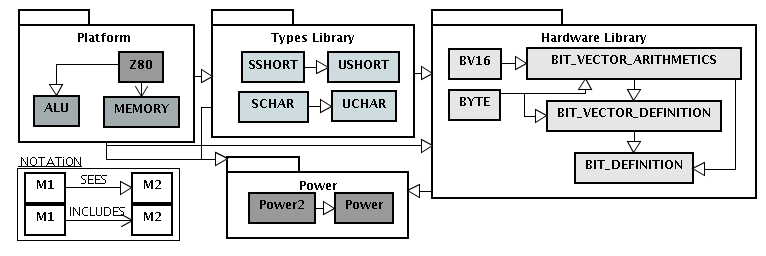
\includegraphics[width=.92\textwidth]{diagramaEstrutural_vertical.png}
 \caption{Dependency diagram of the Z80 model.}
\label{fig:hardware-definition-graph}
\end{figure}



\subsection{Bit representation and manipulation}

The entities defined in the module $\mathit{BIT\_DEFINITION}$ are the
type for bits, logical operations on bits (negation, conjunction,
disjunction, exclusive disjunction), as well as a conversion function
from Boolean to bit.

First, bits are modelled as a set of integers: $\mathit{BIT} =
\mathit{0..1}$. The negation is an unary function on bits and it is
defined as:

$
\begin{array}{l}
\mathit{bit\_not}  \in  \mathit{BIT}  \fun  \mathit{BIT}  \land \forall ( \mathit{bb}). (\mathit{bb} \in \mathit{BIT} \implies \mathit{bit\_not}(\mathit{bb}) =
1-\mathit{bb})\\
\end{array}
$

The module also provides lemmas on negation that may be useful for the
users of the library to develop proofs:

$
\begin{array}{l}
%  \mathit{bit\_not}(0) = 1;  \mathit{bit\_not}(1) = 0; \\
\forall (\mathit{bb}).(\mathit{bb} \in \mathit{BIT} \implies \mathit{bit\_not}(\mathit{bit\_not}(\mathit{bb})) = \mathit{bb})
\end{array}
$

Conjunction is a unary function on bits and it is defined as:

$
\begin{array}{l}
\mathit{bit\_and} \in \mathit{BIT} \times \mathit{BIT} \fun \mathit{BIT} \land \\
\forall (\mathit{b1}, \mathit{b2}).(\mathit{b1}  \in \mathit{BIT}  \land \mathit{b2} \in \mathit{BIT} \implies \\
\quad ((\mathit{bit\_and}(\mathit{b1}, \mathit{b2}) = 1) \iff (\mathit{b1} = 1)  \land  (\mathit{b2} = 1)))
\end{array}
$

The module provides the following lemmas for conjunction, either:

$
\begin{array}{l}
%  \mathit{bit\_and}(0,0) = 0;  \mathit{bit\_and}(0,1) = 0; \\
%  \mathit{bit\_and}(1,0) = 0;  \mathit{bit\_and}(1,1) = 1; \\
\forall (\mathit{b1},\mathit{b2}).(\mathit{b1} \in \mathit{BIT} \land \mathit{b2} \in \mathit{BIT} \implies \\
\quad (\mathit{bit\_and}(\mathit{b1}, \mathit{b2}) = \mathit{bit\_and}(\mathit{b2},\mathit{b1})))\land \\
\forall (\mathit{b1},\mathit{b2},\mathit{b3}).(\mathit{b1} \in \mathit{BIT} \land  \mathit{b2} \in \mathit{BIT} \land \mathit{b3} \in \mathit{BIT} \implies \\
\quad (\mathit{bit\_and}(\mathit{b1}, \mathit{bit\_and}(\mathit{b2},\mathit{b3})) = \mathit{bit\_and}(\mathit{bit\_and}(\mathit{b1},\mathit{b2}),\mathit{b3})))\\
% \forall (\mathit{b1}).(\mathit{b1} \in \mathit{BIT} \implies (\mathit{bit\_and}(\mathit{b1}, 1) = \mathit{b1})); \\
% \forall (\mathit{b1}).(\mathit{b1} \in \mathit{BIT} \implies (\mathit{bit\_and}(\mathit{b1}, 0) = 0));
\end{array}
$

The module provides definitions of $\mathit{bit\_or}$ (disjunction)
and $\mathit{bit\_xor}$ (exclusive disjunction), as well as lemmas on
those operators. These are standard and their expression in B is
similar as for $\mathit{bit\_and}$, they are thus omitted.

Finally, the conversion from Boolean to bit is simply defined as:

$
\begin{array}{l}
\mathit{bool\_to\_bit} \in \BOOL \fun \mathit{BIT} \land \mathit{bool\_to\_bit} = \{ \TRUE \mapsto 1, \FALSE \mapsto 0 \} \\
\end{array}
$

Observe that all the lemmas that are provided in this module have been
mechanically proved by the theorem prover included with our B
development environment. None of these proofs requires human insight.


\subsection{Representation and manipulation of bit vectors}

Sequences are pre-defined in B, as functions whose the domain is an
integer range with lower bound 1 (one). Indices in bit vectors usually
range from 0 (zero) upwards and the model we propose obeys this
convention by making an one-position shift where necessary. This shift
is important to use the predefined functions of sequences. We thus
define bit vectors as non-empty sequences of bits, and
$\mathit{BIT\_VECTOR}$ is the set of all such sequences:
$\mathit{BIT\_VECTOR} = \seq1(\mathit{BIT})$.

The function $\mathit{bv\_size}$ returns the size of a given bit vector. It is basically a wrapper for the
predefined function $\mathbf{size}$ that applies to sequences.

$
\begin{array}{l}
\mathit{bv\_size} \in \mathit{BIT\_VECTOR} \fun \nat_1 \land \\
\mathit{bv\_size} = \lambda bv . (bv \in \mathit{BIT\_VECTOR} \mid \mathbf{size}(bv))
\end{array}
$

We also define two functions $\mathit{bv\_set}$ and $\mathit{bv\_clear}$ that, given a bit vector, and a
position of the bit vector, return the bit vector resulting from setting the corresponding position to 0
or to 1, and a function $\mathit{bv\_get}$ that, given a bit vector, and a valid position, each one
returns the value of the bit at that position. Only the first definition is shown here:


$
\begin{array}{l}
\mathit{bv\_set} \in \mathit{BIT\_VECTOR} \times \nat \fun \mathit{BIT\_VECTOR} \land \mathit{bv\_set} =\\
\lambda v, n . (v \in \mathit{BIT\_VECTOR} \land n \in \nat \land n <\mathit{bv\_size}(v)
\mid v \lover \{ n+1 \mapsto 1 \})
\end{array}
$


The function $bv\_catenate$ takes as parameters two bit vectors $v$ and $w$, and returns the result of the
concatenation of $v$ and $w$, such that $v$ constitutes the most significant part of the result.


% $
% \begin{array}{l}
% \mathit{bv\_catenate} \in \mathit{BIT\_VECTOR} \times \mathit{BIT\_VECTOR} \fun \mathit{BIT\_VECTOR} \land \\
% \mathit{bv\_catenate} = \lambda v, w \bullet (v \in \mathit{ BIT\_VECTOR} \land w \in \mathit{ BIT\_VECTOR}  \mid v 
% %\conc
%   w)
% \end{array}
% $

\hspace*{0.00in} \it bv\_catenate  $\in$  \it BIT\_VECTOR  $\times$  \it BIT\_VECTOR  $\fun$ \it
BIT\_VECTOR $\land$\\
\hspace*{0.00in} \it bv\_catenate \rm =  $\lambda$  v\rm ,\it w \rm . \rm (\it v 
$\in$  \it BIT\_VECTOR $\land$ \it w $\in$  \it BIT\_VECTOR  $\mid$  \it v\^ \it w\rm ) %$\cat$


We also define a function $\mathit{bv\_zero}$ that, given a positive
integer $n$, return a bit vector of size $n$, with all bits set to 0.
A similar function, called $\mathit{bv\_one}$, with all bits set to 1
is also defined but not presented here.

$
\begin{array}{l}
\mathit{bv\_zero} \in \nat_1 \fun \mathit{BIT\_VECTOR} \land \\
\mathit{bv\_zero} = \lambda n \bullet (n \in \nat_1 \mid 1..n \times \{0\}) 
\end{array}
$



Additionally, the module provides definitions for the classical
logical combinations of bit vectors: $\mathit{bit\_not}$,
$\mathit{bit\_and}$, $\mathit{bit\_or}$ and $\mathit{bit\_xor}$. Only
the first two are presented here. Observe that the domain of the
binary operators is restricted to pairs of bit vectors of the same
length:

$
\begin{array}{l}
\mathit{bv\_not} \in \mathit{BIT\_VECTOR} \fun \mathit{BIT\_VECTOR} \land \\
\mathit{bv\_not} = \lambda v . (v \in \mathit{BIT\_VECTOR} \mid \quad \lambda i . (1 .. \mathit{bv\_size}(v)) \mid \mathit{bit\_not}(v(i))) \land \\
\mathit{bv\_and} \in \mathit{BIT\_VECTOR} \times \mathit{BIT\_VECTOR} \fun \mathit{BIT\_VECTOR} \land \\
\mathit{bv\_and} = \lambda v_1, v_2 . (v_1 \in \mathit{BIT\_VECTOR} \land v_2 \in \mathit{BIT\_VECTOR} \land \\
\mathit{bv\_size}(v_1) = \mathit{bv\_size}(v_2) \mid \lambda i . (1 .. \mathit{bv\_size}(v_1)) \mid
\mathit{bit\_and}(v_1(i), v_2(i)))
\end{array}
$

We provide several lemmas on bit vector operations. These lemmas
express properties on the size of the result of the operations
as well as classical algebraic properties such as associativity
and commutativity.

\subsection{Modelling bytes and bit vectors of length 16}

Bit vectors of length 8 are bytes. They form a common entity in
hardware design. We provide the following definitions:


\hspace*{0.0in}\it BYTE\_WIDTH \rm = 8 $\land$ \it BYTE\_INDEX \rm = 1 $\upto$ \rm  BYTE\_WIDTH\rm $\land$

\hspace*{0.0in}\it PHYS\_BYTE\_INDEX \rm = \rm 0 $\upto$ \rm (\it BYTE\_WIDTH\rm -\rm 1\rm )\hspace*{0.10in} $\land$

\hspace*{0.0in}\it BYTE \rm = \rm \{ \it bt  $\mid$  \it bt $\in$ \it BIT\_VECTOR  $\land$  \it bv\_size\rm (\it bt\rm )\rm =\it BYTE\_WIDTH\rm \}\hspace*{0.10in} $\land$

\hspace*{0.0in}\it BYTE\_ZERO  $\in$  \it BYTE  $\land$ \it BYTE\_ZERO \rm = \it BYTE\_INDEX  $\times$  \rm \{\rm 0\rm \}

The $\mathit{BYTE\_INDEX}$ is the domain of the functions modelling bytes. It starts at 1 to obey a
definition of sequences from B. However, it is common in hardware architectures to start indexing from
zero. The definition $\mathit{PHYS\_BYTE\_INDEX}$ is used to provide functionalities obeying this
convention. The $\mathit{BYTE}$ type is a specialized type from $\mathit{BIT\_VECTOR}$, but it has a size
limit. Other specific definitions are provided to facilitate further modelling: the type $\mathit{BV16}$
is created for bit vector of length 16 in a similar way.



\subsection{Bit vector arithmetics}

Bit vectors are used to represent and combine numbers: integer ranges (signed or unsigned). Therefore, our
library includes functions to manipulate such data, for example, the function $\mathit{bv\_to\_nat}$ that
maps bit vectors to natural numbers:



$
\begin{array}{l}
\mathit{bv\_to\_nat} \in \mathit{BIT\_VECTOR} \fun \nat \land \\
\mathit{bv\_to\_nat} = \lambda v . (v \in \mathit{BIT\_VECTOR} \mid \sum i . (i \in \dom(v) . v(i)
\times 2^{i-1}))
\end{array}
$

An  associated lemma is: $\forall n . (n \in \nat_1 \implies \mathit{bv\_to\_nat}(\mathit{nat\_to\_bv}(n)) = n)$

\subsection{Basics data types}

The instruction set of microcontrollers usually have common data types. These types are placed in the
types library. Each type module has functions to manipulate and convert its data. There are six common
basics data types represented by modules, see details in table~\ref{tab:types}.


\begin{table}
\caption{Descriptions of basic data types}
\label{tab:types}

% \begin{center}
% \begin{tabular}{|c|c|c|c|c|c|c|}
% \hline
%  $Type\ Name$ & UCHAR & SCHAR & USHORTINT & SSHORTINT  & BYTE & BV16 \\\hline
%  $Range$ & 0..255 & -128..127 & 0..65.535  & -32.768..32.767  & -- & --\\ \hline
%  $Physical\ Size $ & 1 byte & 1 byte & 2 bytes & 2 bytes &  1 bytes & 2 bytes \\ \hline
% \end{tabular}
% \end{center}

\begin{center}
\begin{tabular}{|c|c|c|c|c|c|c|}
\hline
 $Type\ Name$ & $Range$ & $Physical\ Size $\\\hline
 UCHAR & 0..255 & 1 byte\\\hline
 SCHAR & -128..127 & 1 byte  \\\hline
 USHORTINT & 0..65.535 & 2 byte \\\hline
 SSHORTINT & -32.768..32.767 & 2 byte \\\hline
 BYTE & -- & 1 bytes  \\\hline
 BV16 & -- & 2 bytes \\ \hline
\end{tabular}
\end{center}


\end{table}




Usually, each type module just needs to instantiate concepts that were already defined in the hardware
modelling library.  For example, the function $\mathit{bv\_to\_nat}$ from bit vector arithmetic is
specialized to $\mathit{byte\_uchar}$. As the set $\mathit{BYTE}$ is a subset of the
$\mathit{BIT\_VECTOR}$, this function can defined as follows:


$
\begin{array}{l}
\mathit{byte\_uchar} \in \mathit{BYTE} \fun \nat \land \\
\mathit{byte\_uchar} = \lambda (v) . ( v \in BYTE | bv\_to\_nat(v) )
\end{array}
$

The definitions of the library types reuse the basic definitions from the hardware library. This provides
greater confidence and facilitates the proof process, because the prover can reuse the previously defined
lemma.


The inverse function $\mathit{uchar\_byte}$ is easily defined:

$
\begin{array}{l}
\mathit{uchar\_byte} \in \mathit{UCHAR}  \fun  \mathit{BYTE}  \land \\
   \mathit{uchar\_byte} = \ (\mathit{byte\_uchar}) ^{-1}
\end{array}
$

% We also created the following lemmas:
%
% $
% \begin{array}{l}
%  \forall (val) . (val \in \mathit{UCHAR} |
%  \mathit{byte\_uchar}(\mathit{uchar\_byte}(val)) = val) \land\\
%  \forall (by) . (by \in \mathit{BYTE} |
%  \mathit{uchar\_byte}(\mathit{byte\_uchar}(by)) = by)
% \end{array}
% $
%[NEW PARAGRAPH-TO-REVIEW]
%Similarly, several other general functions and lemmas were created for all other data types.
%Some times, we need create arithmetic and logic functions that are more specific for a
%determined computer architecture. These functions are developed in the module ALU 
%(arithmetic  logic unit). The following shows some examples of specific functions used in
%microcontroller model of Z80. For example, the function $\mathit{instruction_next}$
%receives a $\mathit{BYTE}$ and returns a $\mathit{BYTE}$ that contains a sequence of bit:
%a signal bit, 



\section{A B model of the Z80 instruction set}
\label{sec:z80}

The \textit{Z80} is a CISC microcontroller developed by
\textit{Zilog}~\cite{Z80_manual}. The Z80 is composed by different elements and a
simplified internal organization is shown on the Figure \ref{fig:DiagramBlock}.
This Figure has some important elements of Z80 CPU: ALU, registers of 8 and 16
bits and input/output ports.

\begin{figure}[h] \centering
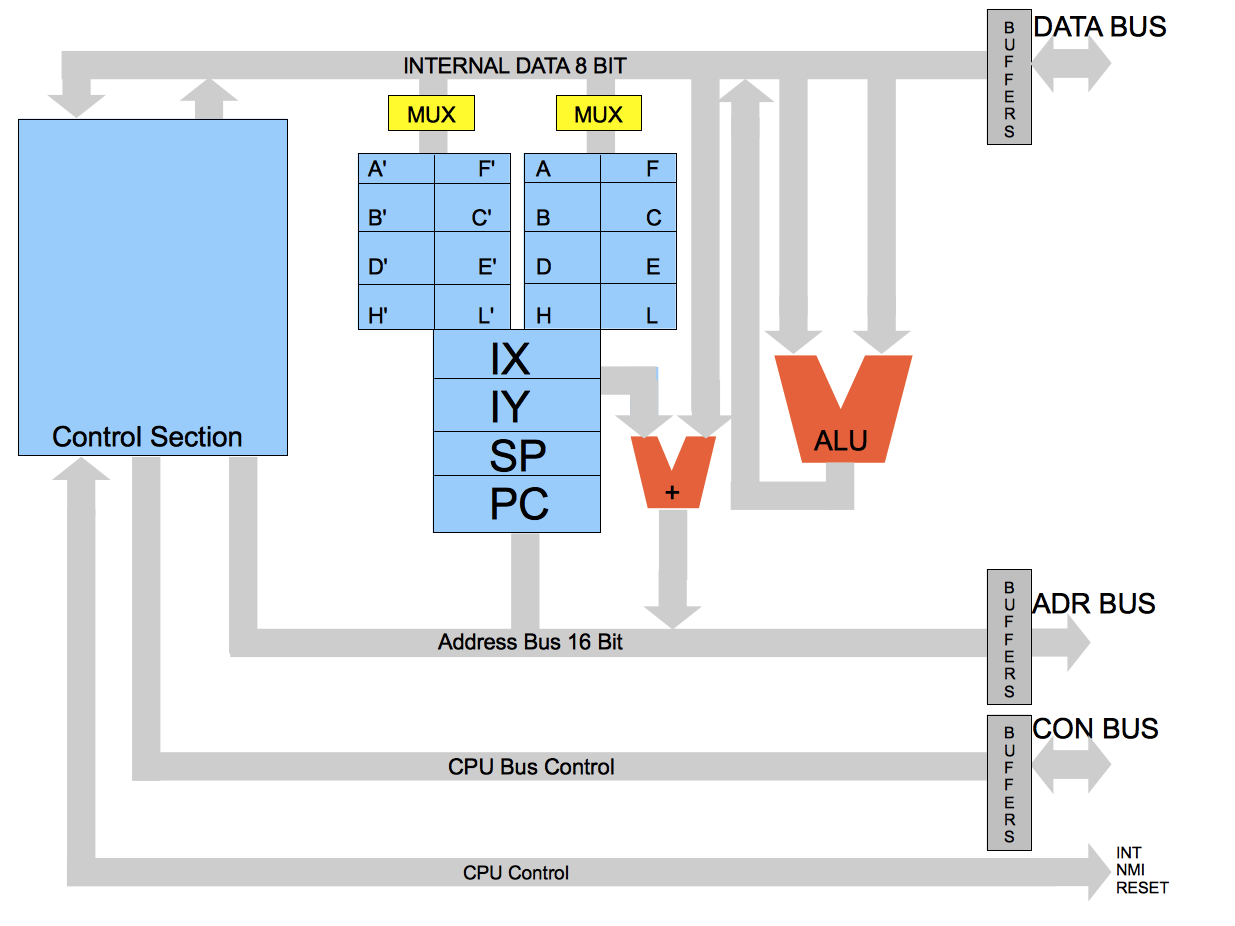
\includegraphics[width=0.78\textwidth]{images/Architecture.png}
\caption{Internal diagram block of Z80 CPU.}
\label{fig:DiagramBlock}
\end{figure}


Z80 supports 158 different instructions, including all the 78 from Intel 8080
microprocessor, and all of them were specified. These instructions are classified
into these categories: load and exchange; block transfer and search; arithmetic
and logical; rotate and shift; bit manipulation; jump, call and return;
input/output; and basic cpu control. Each category of instruction has different
elements of specification.



This section shows the elements that make up the different types of instructions.
The main elements are specified in the microcontroller module Z80 and parts of it
are presented in this section~\ref{sec:z80}. Groups of registers are represented
by the variables of the specification states that appear in clause
\textit{VARIABLES}. The declaration of valid states of variables in the clause is
in the \textit{INVARIANT} clause and the initial state is defined in the
\textit{INITIALISATION} clause. The assembly instructions are defined by the
clause \textit{OPERATIONS}, and the most of its specification constructions are
similar to constructions from traditional programming languages. Several
functions were created to Z80. General functions that can be used in others
microcontroller models are defined in the modules of data types. Specific
functions of the microcontroller are defined in the ULA (arithmetic logic unit).



The main module includes an instance of the memory module and accesses the definitions from basic data
types modules and the \textit{ALU} module.


\begin{sloppypar}

\bf MACHINE

\hspace*{0.15in}\it Z80

\bf INCLUDES

\hspace*{0.10in}\it MEMORY

\bf SEES

\hspace*{0.10in}\it ALU, \it BIT\_DEFINITION, \it BIT\_VECTOR\_DEFINITION,

\hspace*{0.10in}\it BYTE\_DEFINITION, \it BV16\_DEFINITION,

\hspace*{0.10in}\it UCHAR\_DEFINITION, \it SCHAR\_DEFINITION,

\hspace*{0.10in}\it SSHORT\_DEFINITION ,\it USHORT\_DEFINITION
\end{sloppypar}


\subsection{Modelling registers and input and output ports}

The Z80 CPU includes alternative set of accumulator, flag and general registers. The CPU contains a stack
pointer ($\mathit{sp}$), program counter ($\mathit{pc}$), two index registers ($\mathit{ix}$ and $\mathit{iy}$), an
interrupt register ($\mathit{i\_}$), a refresh register ($\mathit{r\_}$), two bits ($\mathit{iff1}$,
$\mathit{iff2}$) used to control the interruptions, a pair of bits to define the interruption mode ($\mathit{im}$)
and the input and output ports ($\mathit{i\_o\_ports}$). Below, its definitions are represented by
\textit{INVARIANT}.
  
\begin{sloppypar}
\bf INVARIANT

\hspace*{0.10in}\it rgs8  $\in$  \it id\_reg\_8  $\fun$  \it BYTE  $\land$ 

\hspace*{0.10in}\it pc  $\in$  \it INSTRUCTION  $\land$  \it sp  $\in$  \it BV16  $\land$  \it ix  $\in$  \it BV16  $\land$  \it iy  $\in$  \it BV16  $\land$ 

\hspace*{0.10in}\it i\_  $\in$  \it BYTE  $\land$  \it r\_ $\in$  \it BYTE  $\land$  

\hspace*{0.10in}\it iff1  $\in$  \it BIT  $\land$ \hspace*{0.10in}\it iff2  $\in$  \it BIT  $\land$ 

\hspace*{0.10in}\it im $\in$ (\it BIT $\times$ \it BIT\rm )  $\land$ 

\hspace*{0.10in}\it i\_o\_ports  $\in$  \it BYTE  $\fun$  \it BYTE
\end{sloppypar}

% 

% Features of microcontroller
 The internal registers contain 176 bits of reading/writing memory that are represented by
identifiers used as parameters in the instructions . It includes two sets of six general purpose
registers which may be used individually as 8-bits registers or as 16-bits register pairs.  The working registers
are represented by variable $\mathit{rgs8}$. The domain of $\mathit{rgs8}$ ($\mathit{id\_regs8}$) is a set
formed by identifiers of registers of 8 bits. These registers can be accessed in pairs, forming 16-bits,
resulting in another set of identifiers of 16-bits registers, named $\mathit{id\_reg16}$.

\begin{sloppypar}
\bf SETS

\hspace*{0.10in}\it id\_reg\_8 \rm = \rm \{ \it a0 \rm , \it f0 \rm , \it f\_0 \rm , \it a\_0 \rm ,

\hspace*{1.0 in}\it b0 \rm , \it c0 \rm , \it b\_0 \rm , \it c\_0 \rm ,

\hspace*{1.00in}\it d0 \rm , \it e0 \rm , \it d\_0 \rm , \it e\_0 \rm ,

\hspace*{1.0in}\it h0 \rm , \it l0 \rm , \it h\_0 \rm , \it l\_0 \} ;

\hspace*{0.10in}\it id\_reg\_16 \rm = \rm \{ \it BC \rm , \it DE \rm , \it HL \rm , \it SP \rm , \it AF \rm \}
\end{sloppypar}

The main working register of Z80 is the accumulator ($\mathit{rgs8(a0)}$) used for arithmetic/logic,
input/output and loading/storing operations.

\subsection{Flag register}
Another important element is the ``f'' register ($\mathit{rgs8(f0)}$),  that is
used as a flag register. This register uses only six bits to represent the execution result status of each instruction.
According to the official manual the bits 3 and 5 are not used and the others bits have the follow meaning:
\begin{description}
  \item[$\mathit{bv\_get(rgs8(f0),0)}$] - The Carry bit
  \item[$\mathit{bv\_get(rgs8(f0),1)}$] - The Add/Subtract bit
  \item[$\mathit{bv\_get(rgs8(f0),2)}$] - The Parity or Overflow bit
  \item[$\mathit{bv\_get(rgs8(f0),4)}$] - The Half Carry bit
  \item[$\mathit{bv\_get(rgs8(f0),6)}$] - The Zero bit
  \item[$\mathit{bv\_get(rgs8(f0),7)}$] - The Sign bit 
\end{description}

These bits also can be used to specify security properties for microcontroller programs.   

\textbf{Assuring the absence of overflow:}
 \emph{To assure that an overflow does not happen, the developer can add this
 expression ($\mathit{bv\_get(rgs8(f0),0)} \neq 1 \land
 \mathit{bv\_get(rgs8(f0),2) \neq 1}$) in the invariant. By default, the overflow
 can happen, but it can be dangerous many times. Then, the developer may
 prohibit its use. This restriction can also become more difficult to specify
 the instructions.}



\subsection{Manipulation data functions from Z80}
 There are some specific functions
from Z80 to manipulate the data. In addressing mode, the function
$\mathit{bv\_ireg\_plus\_d}$ is  used to indexed address. It receives the value
of register ($\mathit{ix}$ or $\mathit{iy}$) and the displacement to return the
sum, the result is the dislocated address memory, see its definition.

\hspace*{0.0in}\it bv\_ireg\_plus\_d \rm : \rm(\it BV16  $\times$  \it SCHAR  $\fun$  \it BV16\rm )  $\land$ 

\hspace*{0.0in}\it bv\_ireg\_plus\_d \rm =  $\lambda$  \rm ( \it ix\_iy \rm , \it disloc \rm ) \rm . \rm ( \it ix\_iy  $\in$  \it BV16  $\land$  \it disloc  $\in$  \it SCHAR   

\hspace*{0.20in}$\mid$ \it ushort\_bv16 \rm ( \rm (\it bv16\_ushort \rm ( \it ix\_iy \rm ) \rm + \it disloc \rm ) 
$\mod$ \rm 6\rm 5\rm 5\rm 3\rm 6 \rm ) \rm )

Another derived function is  $\mathit{bv\_(ireg\_plus\_d)}$, this returns the value in the memory  address
returned by $\mathit{bv\_ireg\_plus\_d}$ function and its definition is similar.

There is a specific function to refresh the flag register, it is named $\mathit{update\_reg\_flag}$. It is typed of
follow mode: \it update\_flag\_reg \rm $\in$ \rm (\it BIT  $\times$  \it BIT  $\times$  \it BIT  $\times$  \it
BIT $\times$  \it BIT  $\times$  \it BIT\rm) $\fun$  \rm (\rm \{\it f0\rm \}  $\times$  \it BYTE\rm ). 

\it update\_flag\_reg \rm =  $\lambda$  \rm (\it s7 \rm, \it z6 \rm,\it h4 \rm,\it pv2 \rm ,\it n1
\rm ,\it c0 \rm)$\bullet$

\rm ( \it s7 $\in$ \it BIT $\land$ \it z6 $\in$ \it BIT $\land$ \it h4 $\in$ \it
BIT $\land$ \it pv2 $\in$ \it BIT $\land$ \it n1 $\in$ \it BIT $\land$ \it c0 $\in$ \it BIT
  
\hspace*{0.20in}\rm $\mid$( \it f0  $\mapsto$  \rm \rm [\it c0\rm , \it n1\rm , \it pv2\rm , \rm 1\rm , \it
h4\rm , \rm 1\rm , \it z6\rm , \it s7\rm \rm ]\rm ) \rm )


\subsection{Program, stack and data memory}

The Z80 uses a unique memory for storing program instructions, data stack and
data work. The memory has 16-bits address and each address represents a byte.
Thus, the data from the memory module is very simple, as shown below, but an
additional care must be taken to preserve the memory consistency.

\begin{sloppypar}
\bf INVARIANT \\
\hspace*{0.10in}\it mem  $\in$  \it BV16  $\fun$  \it BYTE 

\end{sloppypar}
  
In general, the instructions can access all memory address, but it is very
dangerous. For adding more security, it is important that the program
instructions has the limited access by region. Thus the designer can specify
address regions to restrict the access from instructions. The address regions can
be specified how shown below. The constants
($\mathit{PRORGRAM\_R\_ADR,DATA\_R\_ADR,STACK\_R\_ADR}$) defines respectively a
range of restricted address for: programs instructions, data work, data stack.

$
\begin{array}{l}
\mathit{PROGRAM\_R\_ADR} = 0..16384 \land\\
\mathit{DATA\_R\_ADR} = 16385..49151 \land\\
\mathit{STACK\_R\_ADR} = 49152..65535
\end{array}
$

\textbf{Assuring the absence of overlapping of address regions:}
 \emph{To assure that address regions are well defined, then the designer must to verify the below expression.}

\begin{sloppypar}
\hspace*{0.10in}\it PROGRAM\_R\_ADR $\cap$ DATA\_R\_ADR $\cap$  STACK\_R\_ADR $=$ \{\}
\end{sloppypar}
 
\textbf{Preserving the consistency of the memory:} \emph{In general, the access to
some address regions is dangerous. Then, in each instruction has a specific pre-condition that verify
if the new address memory, that will be updated, is member of its region. For example, the $\mathit{PUSH}$
program instruction allows write only in the region of stack ($\mathit{STACK\_R\_ADR}$).}



\subsection{Arithmetic logic unit}
 
There are many functions defined in the module \textit{ALU}. In general, these functions take basic definitions or functions
to build new more specific functions. The function $\mathit{half8UCHAR}$ is used to get the half part of $\mathit{UCHAR}$ value.
It is important to know the half carry and it is used in the function $\mathit{add8UCHAR}$. 

\hspace*{0.0in}

\hspace*{0.0in}\it half8UCHAR  $\in$  \it UCHAR  $\fun$  \it UCHAR  $\land$ 

\hspace*{0.0in}\it half8UCHAR \rm =  $\lambda$  \rm (\it ww\rm )\rm .\rm (\it ww  $\in$  \it UCHAR  $\mid$  \it ww  $\mod$  \it $2^{4}$\rm )

\hspace*{0.0in}

 
The function $\mathit{add8UCHAR}$ receive a bit carry and two $\mathit{UCHAR}$ values and return respectively the 
sum, the sign bit, the carry bit, the half carry bit and the zero bit. It is typed how follow: \it add8UCHAR \rm :
\rm (\it BIT $\times$ \it UCHAR $\times$ \it UCHAR\rm ) $\fun$ \rm (\it UCHAR $\times$  \it BIT  $\times$  \it BIT  $\times$  \it BIT  $\times$  \it BIT\rm ) and its definitions is:

\hspace*{0.0in}\it add8UCHAR\rm = $\lambda$ \rm(\it carry\rm,\it w1\rm \it w2\rm)\rm.\rm

\hspace*{0.0in}(\it carry $\in$  \it BIT  $\land$  \it w1  $\in$  \it UCHAR  $\land$  \it w2  $\in$  \it UCHAR
$\mid$

\hspace*{0.40in}\rm(\rm(\rm(\it carry \rm + \it w1 \rm + \it w2 \rm )  $\mod$  \it $2^{8}$ \rm ),

\hspace*{0.40in}\it bool\_bit\rm ( \it carry \rm + \it uchar\_schar\rm (\it w1\rm ) \rm + \it uchar\_schar \rm (\it
w2\rm ) $<$ \rm 0\rm ),

\hspace*{0.40in}\it bool\_bit\rm ( \it carry \rm + \it w1 \rm + \it w2 $>$ \it UCHAR\_MAX\rm )\rm ,

\hspace*{0.40in}\it bool\_bit\rm ( \it carry \rm + \it half8UCHAR\rm (\it w1\rm ) \rm + \it half8UCHAR\rm ( \it
w2\rm )  $\geq$  \it $2^{4}$\rm )\rm,

\hspace*{0.40in}\it bool\_bit\rm ( \rm ( \rm (\it carry \rm + \it w1 \rm + \it w2 \rm )  $\mod$  \it $2^{8}$ \rm
)\rm = \rm 0\rm )\rm )\hspace*{0.10in}\rm )

\hspace*{0.20in}

A related function to subtract operation is $\mathit{substract8UCHAR}$. There are the same functions for the
$\mathit{SCHAR}$ type, they are respectively $\mathit{add8SCHAR}$ and $\mathit{substract8SCHAR}$, all these
functions are of 8 bits ($\mathit{BYTE}$) and defined similarly. In the same way, the arithmetic functions for 16
bits ($\mathit{BV16}$) are defined.
The module ALU has several others functions, but only some simplest functions also are typed and explained below:

\begin{itemize}
  %\item \it inc  $\in$ \it BYTE $\fun$  \it BYTE \rm - It receives a byte and
  %returns its increment. There is a similar function named $\mathit{dec}$.

  \item \it instruction\_next  $\in$  USHORT  $\fun$  USHORT \rm - It receives the  
  actual value from program counter register (\textit{pc}) and returns its increment.
 \item \it is\_negative  $\in$  \it BYTE  $\fun$  \it BIT \rm - It returns the most significant bit,
 in other words, the signal bit.

  
 % \item \it is\_zero  $\in$  \it BYTE  $\fun$  \it BIT \rm - It returns 1 if the received
 % byte is zero, otherwise returns 0.

  %\item \it update\_refresh\_reg \rm - It receives a byte and returns its increment until the seventh bit.

\end{itemize}

The logic functions that are defined in the \textit{BYTE} and \textit{BV16}
module are included in the \textit{ALU} module. Then, these functions can be seen
directly in the \textit{ALU} and \textit{Z80} module.

\subsection{Modelling the instructions}

Each instruction is represented by a B operation in the module Z80. The main
module (\textit{Z80}) has two types of operations, a type represents the external
actions and the other represents the instructions of microcontrollers. The
external actions are shown in the section ~\ref{sec:externalactions}.  A simple
example from instruction is a
$\mathit{LD\_(nn)\_A}$\footnoteremember{myfootnote}{The tools B does not allow
to use parentheses in identifiers, then the characters \{``('',``)''\} are
replaced respectively by \{``9'',``0''\} in the real specification.} shown below. The
pre-defined functions is necessary many times to model the instructions, this
functions facilitates the construction of instruction set model. By default, all
parameters from operations are either predefined elements in the model or
integers values in the decimal representation. This instruction use the
$\mathit{updateAddressMem}$ function from \textit{Memory} module and it receives
a address memory and its new memory value. After, it increments the program
counter ($\mathit{pc}$) and update the refresh register ($\mathit{r\_}$).


\hspace*{0.00in}\bf LD\_9nn0\_A \rm ( \it nn \rm ) \rm =

\hspace*{0.20in}\bf PRE \it nn $\in$ \it USHORT\hspace*{0.15in} $\land$ \hspace*{0.10in}\it nn\hspace*{0.10in} $\in$  \it DATA\_R\_ADR

\hspace*{0.20in}\bf THEN

\hspace*{0.20in}\bf updateAddressMem \rm ( \it ushort\_bv16 \rm ( \it nn \rm ) \rm , \it rgs8 \rm ( \it a0 \rm )
\rm )  $\para$

\hspace*{0.20in}\it pc \rm := \it instruction\_next \rm ( \it pc \rm )  $\para$  \it r\_ \rm := \it update\_refresh\_reg\rm (\it r\_\rm )

\hspace*{0.00in}\bf END\rm ;

The other instructions have a similar structure.

\subsection{Modelling the input/output instructions}

The Z80 has an extensive set of input and output (I/O) instruction and 256 ports for
devices. This model can transfer data blocks and between the I/O devices and any
of the internal registers or memory address.

The $\mathit{IN\_r(C)}$\footnoterecall{myfootnote} instruction is represented
by the following B operation. It is from I/O group, then it receives an
identifier of register $\mathit{r}$ and, in this place, it stores the value of $\mathit{C}$ port address. Besides, it increments the
program counter and updates the flag registers.

\hspace*{0.0in}\bf IN\_r\_9C0 \rm ( \it rr \rm ) \rm =

\hspace*{0.0in}\bf PRE \it rr  $\in$  \it id\_reg\_8  $\land$  \it rr  $\not =$  \it f0\hspace*{0.15in}\bf THEN

\hspace*{0.20in}\bf ANY

\hspace*{0.40in}\it negative \rm , \it zero \rm , \it half\_carry \rm , \it pv \rm , \it add\_sub \rm , \it carry

\hspace*{0.20in}\bf WHERE 

\hspace*{0.40in}\it negative $\in$ \it BIT $\land$ \it zero $\in$ \it BIT $\land$ \it half\_carry $\in$ \it BIT 
$\land$ \it pv $\in$ \it BIT $\land$

 \hspace*{0.40in}\it add\_sub $\in$ \it BIT $\land$ \it carry $\in$ \it BIT  $\land$

\hspace*{0.40in}\it negative \rm = \it is\_negative \rm ( \it io\_ports \rm ( \it rgs8 \rm ( \it c0 \rm ) \rm ) \rm )  $\land$ 

\hspace*{0.40in}\it zero \rm = \it is\_zero \rm ( \it io\_ports \rm ( \it rgs8 \rm ( \it c0 \rm ) \rm ) \rm )  $\land$ 

\hspace*{0.40in}\it half\_carry \rm = \rm 0  $\land$ 

\hspace*{0.40in}\it pv \rm = \it parity\_even \rm ( \it io\_ports \rm ( \it rgs8 \rm ( \it c0 \rm ) \rm ) \rm ) $\land$

\hspace*{0.40in}\it add\_sub \rm =\hspace*{0.10in}\rm 0  $\land$ 

\hspace*{0.40in}\it carry \rm = \it z\_c

\hspace*{0.20in}\bf THEN

\hspace*{0.40in}\it rgs8 \rm := \it rgs8  $\lover$  \rm \{ \rm ( \it rr  $\mapsto$  \it io\_ports \rm ( \it rgs8 \rm ( \it c0 \rm ) \rm ) \rm ) \rm ,

\hspace*{0.40in}\it update\_flag\_reg\rm (\it negative\rm,\it zero\rm,\it half\_carry\rm,\it pv\rm,\it add\_sub\rm,\it carry)\rm\}$\para$

\hspace*{0.40in}\it pc \rm := \it instruction\_next \rm ( \it pc \rm )  $\para$  \it r\_ \rm := \it update\_refresh\_reg\rm (\it r\_\rm )

\hspace*{0.0in}\bf END \rm

The main I/O instructions work similarly, for example: $\mathit{OUT(n),A}$  or
$\mathit{OUT (C ), r}$. There are several other instructions of I/O, besides,
these ones are the most commonly used.

% $
% \begin{array}{l} 
% \mathit{IN\_r\_9C0} ( rr ) = \\
% \quad   \PRE rr \in id\_reg\_8    \THEN\\
% \quad\quad \ANY data\_in, negative , zero , half\_carry , pv , add\_sub , carry\\ 
% \quad\quad \WHERE data\_in \in \mathit{BYTE} \land negative \in \mathit{BIT}\land\\
% \quad\quad\quad carry \in \mathit{BIT} \land half\_carry \in \mathit{BIT} \land zero \in \mathit{BIT} \land \\
% \quad\quad\quad negative = is\_negative (data\_in) \land zero = is\_zero(data\_in ) \land\\
% \quad\quad\quad half\_carry = 0 \land pv =parity\_even\_BYTE ( data\_in )    \land\\
% \quad\quad\quad add\_sub =  0 \land carry = z\_c \\
% \quad\quad  \THEN \\
% \quad\quad\quad i\_o\_ports ( rgs8 ( c0 ) ) := data\_in ||\\
% \quad\quad\quad rgs8 := rgs8 <+ \{ ( rr |-> data\_in ) ,\\
% \quad\quad\quad get\_new\_flag\_register\_SZ\_H\_PvNC ( rgs8 , negative , zero, half\_carry , pv , add\_sub , carry ) \} ||\\
% \quad\quad\quad pc := instruction\_next( pc )\\
% \quad\quad \END\\
% \quad \END\\
% \end{array}
% $




\subsection{Modelling the external actions}
\label{sec:externalactions}

The external actions change the state of microcontroller and they are not
instructions, for example, the refreshing of I/O port and the interruptions
request. The external actions are also model by operations and they are named with the
prefix ``$ext\_$'' and after the name of action. There are just four external
actions: $ext\_update\_io\_ports$, $ext\_NMI$ and $ext\_INT$, $ext\_Reset$. The
$ext\_update\_io\_ports$ just change the state of I/O port, see.

\hspace*{0.20in}\bf ext\_update\_io\_ports\rm (\it address\rm ,\it value\rm )\rm =

\hspace*{0.20in}\bf PRE \it address  $\in$  \it UCHAR  $\land$ \hspace*{0.10in}\it value  $\in$  \it SCHAR \bf THEN

\hspace*{0.40in}\it io\_ports \rm ( \it uchar\_byte \rm ( \it address \rm ) \rm ) \rm := \it schar\_byte \rm ( \it
value \rm )

\hspace*{0.20in}\bf END\rm 

The other external actions are related to interruptions. The interruptions allow
that the devices suspend a routine from CPU and start another service routine.
This service routine can exchange data or signals between CPU and external
devices. When a routine is finished, then the CPU comes back to the last routine
that was interrupted.

For the interrupts, the following things are important:  the interrupt flip-flops
($\mathit{iff1}$ and $\mathit{iff2}$), the types of interrupts (maskable and
non-maskable), the interrupt mode (set with the $\mathit{IM 0}$, $\mathit{IM 1}$,
$\mathit{IM 2}$ instructions) and the $\mathit{i\_}$ register.

The $\mathit{iff1}$ and $\mathit{iff2}$ control the maskable interrupts
($\mathit{INT}$). When the $\mathit{iff1}$ is set, the interrupt is enabled,
otherwise it is disabled. The $\mathit{iff2}$ is used only as a temporay storage
place for $\mathit{iff1}$. The $\mathit{iff1}$ is 1 or 0 by instructions
$\mathit{EI}$ and $\mathit{DI}$, that respectively enable and disable the
maskable interruptions.


The interruptions and the \textit{reset} action change the state of
microcontroller. Theses actions are modelled by B operations and the its main
effects are shown below\footnote{Some definitions of constants: $\mathit{sp\_minus\_two}$ is the value of stack pointer minus 2,
%=$\mathit{dec\_BV16(dec\_BV16(sp))}$
 $\mathit{sp\_minus\_one}$ is the value of stack pointer minus 1,
%=$\mathit{dec\_BV16(sp)}$
$\mathit{pc\_high}$ is the most significant 8 bits and
$\mathit{pc\_low}$ is the others least significant.}.


 \textbf{NMI} - Non-maskable interrupts - The non-maskable cannot be disabled
 by the programmer. Then, when a device makes a request, the $sp$ is pushed, the
 $pc$ receives $66H$ (102 in decimal), the $\mathit{iff1}$ is reset , $\mathit{iff2}$ stores
 $\mathit{iff1}$ and refresh register is updated.
  
\begin{sloppypar}
\bf updateStack\rm (\rm \{ \rm (\it sp\_minus\_two  $\mapsto$  \it pc\_low\rm )\rm ,\rm (\it sp\_minus\_one  $\mapsto$ \it pc\_high \rm ) \rm \}\rm )$\para$

\it sp \rm := \it sp\_minus\_two  $\para$ \it pc \rm := \rm 1\rm 0\rm 2 $\para$ \it iff1\rm :=\rm 0  $\para$  \it iff2\rm := \it iff1 $\para$

\it r\_ \rm := \it update\_refresh\_reg\rm (\it r\_\rm )\\
\end{sloppypar}

  \textbf{INT} - Maskable Interrupt -  This is usually reserved to important functions that can be enabled and
  disabled by the programmer. When a maskable interrupt action happens, both $\mathit{iff1}$ and $\mathit{iff2}$ are
  cleared, disabling the interrupts, the $sp$ is pushed, the refresh register is updated  and the other effects
  depend on the interrupt mode (\it im \rm).
 

 \begin{itemize}
   
  \item The mode 0 is compatible with 8080 and  \it im \rm = \rm ( \rm 0 $\mapsto$  \rm 0 \rm ). When a 
  non-maskable interruption happens, the CPU fetches an instruction of one byte
  from an external device, usually an RST instruction, and the CPU executes it.
  The instruction code is received from an external device by data bus and it is represented by integer parameter called $\mathit{byte\_bus}$ .

 
  \item The mode 1 is the easiest and \it im \rm = \rm ( \rm 0  $\mapsto$  \rm 1
  \rm ). Simply, when a non-maskable interruption happens, the program counter
  receives $38H$ (56 in decimal).
  
  \item The mode 2 is the most flexible and  \it im \rm = \rm ( \rm 1  $\mapsto$
  \rm 1 \rm ). When a non-maskable interruption happens, an indirect call can be
  made to any address memory. The program counter receives a bit vector of size
  16 composed with two parts: the most significant part of the $\mathit{i\_}$
  register and the least significant part of the $\mathit{byte\_bus}$ with the
  last bit cleared.
 \end{itemize}

The essential part of maskable interrupt is shown below\footnote{ The
 $\mathit{byte\_bus}$ is parameter from  $\mathit{INT}$ operation }. 
 


\begin{sloppypar}

\hspace*{0.00in}\bf IF \it im \rm = \rm ( \rm 0  $\mapsto$  \rm 0 \rm ) \bf THEN  

\hspace*{0.10in}\bf IF\hspace*{0.10in}\it byte\_bus \rm $\in$  \it opcodes\_RST\_instruction

\hspace*{0.10in}\bf THEN\hspace*{1.05in}

\hspace*{0.40in}\it pc \rm := \it byte\_bus \rm - \rm 1\rm 9\rm
9\hspace*{0.10in} $\para$

\hspace*{0.40in}\bf updateStack\rm ( \rm \{ \it stack\rm ( \it
sp\_minus\_one\rm )  $\mapsto$  \it pc\_low\rm ,

\hspace*{0.40in}\it stack\rm (\it sp\_minus\_two\rm )  $\mapsto$  \it pc\_high
\rm \} \rm )  $\para$

\hspace*{0.40in}\it sp \rm := \it sp\_minus\_two  $\para$ \hspace*{0.10in}\it
r\_ \rm := \it update\_refresh\_reg\rm (\it r\_\rm )

\hspace*{0.10in}\bf ELSIF \it byte\_bus \rm = \it opcode\_\ldots\_instruction

\hspace*{0.40in}\bf \ldots 

\hspace*{0.10in}\bf END

\hspace*{0.00in}\bf ELSIF\hspace*{0.10in}\it im \rm =\hspace*{0.10in}\rm ( \rm
0  $\mapsto$  \rm 1 \rm ) \bf THEN

\hspace*{0.10in}\it pc \rm :=\hspace*{0.10in}\rm 5\rm 6  \hspace*{0.80in}
$\para$

\hspace*{0.10in}\bf updateStack\rm ( \rm \{ \it stack\rm (\it
sp\_minus\_one\rm )  $\mapsto$  \it pc\_low\rm ,

\hspace*{0.10in}\it stack\rm (\it sp\_minus\_two\rm )  $\mapsto$  \it pc\_high
\rm \} \rm )  $\para$

\hspace*{0.10in}\it sp \rm := \it sp\_minus\_two  $\para$ \hspace*{0.10in}\it
r\_ \rm := \it update\_refresh\_reg\rm (\it r\_\rm )\hspace*{0.85in}

\hspace*{0.00in}\bf ELSIF\hspace*{0.10in}\it im \rm = \rm ( \rm 1  $\mapsto$ 
\rm 1 \rm ) \bf THEN  \hspace*{0.70in}

\hspace*{0.10in}\it pc \rm := \it bv16\_ushort\rm (\it byte\_bv16\rm ( \it i\_
\rm ,\it bv\_clear\rm (\it rotateleft\rm (\it uchar\_byte\rm (\it byte\_bus\rm )\rm )\rm ,\rm 0\rm )\rm )\rm )$\para$

\hspace*{0.10in}\bf updateStack\rm ( \rm \{ \it stack\rm ( \it
sp\_minus\_one\rm )  $\mapsto$  \it pc\_low\rm ,

\hspace*{0.10in}\it stack\rm (\it sp\_minus\_two\rm )  $\mapsto$  \it pc\_high
\rm \} \rm )  $\para$

\hspace*{0.10in}\it sp \rm := \it sp\_minus\_two  $\para$ \hspace*{0.10in}\it
r\_ \rm := \it update\_refresh\_reg\rm (\it r\_\rm )

\hspace*{0.00in}\bf END\hspace*{0.10in}\\
\end{sloppypar}


\textbf{RESET}  - This just reset the registers related to the interruptions.

\begin{sloppypar}
\it iff1 \rm :=\rm 0 $\para$ \it iff2\rm :=\rm 0 $\para$  \it  im\rm := \rm (\rm 0 $\mapsto$ \rm 0\rm )  $\para$ 
\it pc\rm :=\rm 0 $\para$ \it i\_ \rm := [0,0,0,0,0,0,0,0] $\para$

\it rgs8 \rm := \it rgs8  $\lover$  \rm \{ \rm (\it a0  $\mapsto$ \rm [0,0,0,0,0,0,0,0] , \rm (\it
f0 $\mapsto$ \rm [0,0,0,0,0,0,0,0] \rm \} $\para$

\it r\_  \rm := [0,0,0,0,0,0,0,0] $\para$ \it sp \rm := [0,0,0,0,0,0,0,0,0,0,0,0,0,0,0,0]
\end{sloppypar}


%The microcontroller model can specify security properties. For example, the
%last operation could have a restriction to write only in a defined region of memory.


\subsection{Considerations about the Z80 model}


The Z80 formal model provides many benefits, because of the verification of
generated proof obligations assure: the correct use of data types, the developed
security properties  and if the expressions used are well-defined
(WD)\footnote{An expression is called ``well-defined'' (or unambiguous) if its definition assigns
it a unique interpretation or value.}. Furthermore, the designer has a big
flexibility to create new and specific security properties, this is very useful
to adjust the verification in accordance with the requirements. Moreover, this
example of model could replace or improve the used documentation for users and
assembly programmers. Z80 model is also useful to develop verified software 
up to the assembly level. There are many benefits when a formal model is
developed, but to verify completely the model is not an easy task and more
details are shown in section~\ref{sec:Verification}. Finally, the next section explains
a verified case study since the first abstract B model up to B
assembly model.

\section{Building and verifying assembly-level refinements}
\label{sec:studycase}


This section shows a case study that carries an out experimental evaluation of
a pilot project with B refinements until the assembly level. The object of
the pilot project was developed to analyse a petroleum production test system.  

%A seção 1 apresenta uma introdução sobre o sistema de teste de produção em tanque e a seção seguinte
%descreve a modelagem B e B \textit{assembly}. A seção 3 mostra a simulação do \textit{software}
%desenvolvido, o que foi realizado para testar o seu funcionamento. Finalmente, a última seção 
%apresenta as considerações finais sobre a modelagem desse estudo de caso.


\subsection{Petroleum production test system}

%\subsection{Teste de produção em tanque}

% Intro % O que é isso ?
%O teste de produção é ``o processo usado para o acompanhamento do desenvolvimento da produção de um
%campo de petróleo, o qual é executado em cada poço deste campo numa frequência previamente definida''
%\cite{LAUT_SERGIO}. Nesse processo são analisadas as características do óleo, gás e água extraídos, tais como:
%volume, concentração de água, temperatura, entre outras.	

The production test is ``the process used to  monitor the production of an oil
field, this process is executed in each oil field in a predefined frequency''
according to \cite{LAUT_SERGIO}. In this process, some characteristics
are analysed (concentration of water, volume and temperature) from oil, gas and
water.

%% Porque modelar isso ? O que pode melhorar ?
%Esse tipo de teste possui um papel importante no processo de extração. Ele é fundamental
%para avaliar a capacidade de extração dos poços e para designar o pagamento dos impostos governamentais, o pagamento de \textit{royalties} aos
%municípios, as participações especiais e as participações aos proprietários de terra. No entanto,
%atualmente, segundo registros dos testes no sistema de informação, 10\% deles são falhos~\cite{LAUT_SERGIO}. Logo, é importante que
%esses testes obtenham a melhor precisão possível, a fim de garantir uma melhor qualidade, credibilidade e
%transparência.


This production test system has an important purpose in the process of oil
extraction. It is required to analyse the production capacity of wells and
calculate the government taxes, special participations and participations for
landowners. However, based on the registers of the information system test,
10\% of production tests are failed tests~\cite{LAUT_SERGIO}. So, we have developed an embedded
software verified until the assembly level to help the production test. Actually,
the developed software is simplified, because its main objective is to evaluate
and to improve the verification up to the assembly level.



% Simplificação/abstração de detalhes não relevantes
%O sistema de teste de produção é utilizado para controlar e avaliar a produção de petróleo. Ele possui um
%sistema supervisório que calcula a produção de petróleo e controla as válvulas de acordo com os estados do
%sistema, do sensor de interface e do radar. O radar informa o nível total do fluido no tanque e o
%sensor de interface informa a concentração de água na emulsão em um ponto local independente da
%densidade, viscosidade e temperatura de operação, o que ajuda a identificação do nível da interface. Esse sistema é complexo
%e pode ser considerado sob vários pontos de vista, no entanto, ele é simplificado nessa proposta até o nível de abstração
%adequado para facilitar o entendimento. 

%Uma série de técnicas e cuidados físicos deve ser aplicada para realização correta dos testes de produção. Dessa forma, o sistema de teste
%envolve uma considerável complexidade. Além disso, os trabalhos de~\cite{LAUT_SERGIO,LAUT_LIMA} definem vários
%detalhes físicos e parámetros para melhorar a qualidade dos testes, os quais foram obtidos e aprimorados após
%experimentos em campo. Esses detalhes podem ser consultados nos trabalhos citados, e nesse trabalho é
%apresentada apenas uma visão geral do problema e a especificação de uma parte do sistema.

The production test system is used to control and to evaluate the oil production.
It has a system supervisor that calculates the oil production and controls the
valves based on the state of system and information from sensor interface and
radar. The radar informs the total level of fluid in the tank and the interface sensor
informs the concentration of water in oil that helps to identify the level of
interface oil and water.
% Several physical precautions and techniques can be applied to execute correctly
% the production system test.




% % Como funciona o estudo de caso?
% O teste de produção, resumidamente, possui três fases de acordo
% com~\cite{LAUT_SERGIO}. Primeiramente, inicia a fase de condicionamento, o
% sistema de controle do tanque é atualizado com dados coletados do último teste,
% o sistema mantêm o poço alinhado\footnote{Um poço está alinhado quando as
% válvulas da tubulação direcionam o fluxo do poço para o tanque.} e ao final dessa fase a válvula de drenagem é fechada.


The production test has basically three stages according to~\cite{LAUT_SERGIO}.
First, the conditioning stages begin, the control system of the tank is updated
with data collected from the last test, the system keeps the well
aligned\footnote{A well is aligned when the valves direct the flow pipe from the
well to the tank.} and the drain valve is closed in the end of this stage.

% Em seguida, inicia a fase de enchimento e decantação, logo após o enchimento e
% a espera, que pode variar de 8 a 20 horas de decantação, começa a fase de
% drenagem. Nessa última fase, o sistema deve
% controlar a válvula de drenagem para não permitir fluir o óleo extraído e calcular a sua quantidade.
% E esse cálculo é o objeto de interesse do presente estudo de caso.

Then the process of filling and decanting begins. After filling and waiting,
which can wait between 8 and 20 hours of decanting, the draining stage begins.
The draining stage is on that last one stage, the system must control the drain valve
not to allow the extracted oil to flow and to estimate final quantity oil. Only
the calculus used to estimate oil quantity in this last stage is important to the
case study verified up to assembly level.

%As três fases citadas são exibidas na mesma ordem na Figura~\ref{fig:CaseStudy}. Nessa figura é
%possível observar os dispositivos utilizados no teste de produção e os estados do tanque
%em cada fase.
The three stages are shown, in the same sequence, in Figure~\ref{fig:CaseStudy}.
In this Figure, it is also possible to see the used devices in the production
test.

\begin{figure}[h] \centering 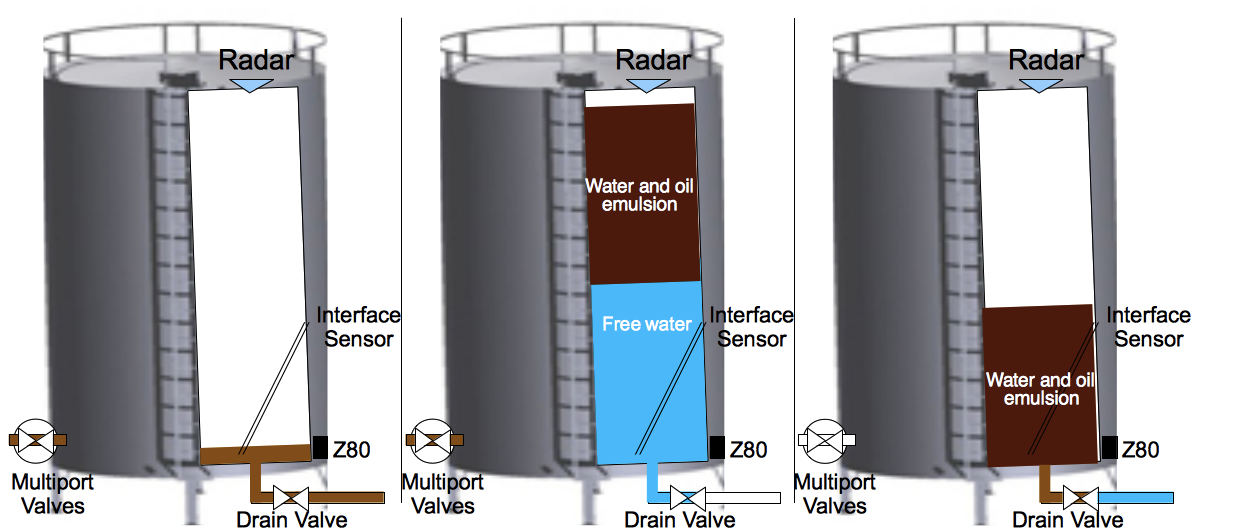
\includegraphics[width=1.\textwidth]{images/FasesEstudoDeCaso.png}
\caption{Stages of the production test.}
\label{fig:CaseStudy}
\end{figure}

% Na fase de drenagem, o nível de óleo desce relativamente rápido até aproximar-se do sensor de interface.
% Nesse instante a válvula de drenagem começa a fechar lentamente e, consequentemente, diminui a
% velocidade de  saída do fluido. Todo esse cuidado é importante para evitar a formação de vórtice\footnote{Vórtice
% é disposição concêntrica e raiada do fluido, ou seja, redemoinho ou pequenas
% ondas.}, o que afeta diretamente as propriedades do óleo extraído.


% [Dúvidas]
% - O sistema de automação usa clp (microcontrolador), ok? Sim Onde? No controle da válvulas, no recebimento das
% informações e cálculo de nível. Mais detalhes podem ser obtidos na dissertacao de LIMA
% - O  computador supervisório ? Apenas monitora e envia comandos! O microcontrolador é quem trabalha mesmo! Mais
% metalhes na {LAUT_LIMA}
% - 

%\begin{figure}[h]
%\centering 
%\includegraphics[width=.8\textwidth]{images/fluxograma_teste_drenagem.png}
%\includegraphics[width=0.95\textwidth]{images/diagrama_de_atividades.png}
%\caption{Diagrama de atividades do sistema de controle da válvula de drenagem do teste de produção
%\cite{LAUT_SERGIO}.}

%\label{fig:FluxogramaEstudoDeCaso}
%\end{figure}

%A Figura~\ref{fig:FluxogramaEstudoDeCaso} mostra o diagrama de atividades sobre o sistema de controle da
%válvula de drenagem.
% Contudo, para melhor entender o diagrama é necessário conhecer alguns conceitos: BSW
%é a abreviação de \textit{Basic Sediments and Water} e mede a proporção de água e sedimentos no fluído
%extraído; BSWe mede a proporção do volume de água contido na emulsão água e óleo entre o volume total
%dessa emulsão; CW (\textit{cut water}) representa a capacidade do óleo emulsionado reter mais ou menos
%água. De acordo com \cite{LAUT_SERGIO}, o CW é definido no programa como 20\% ou 40\%, conforme a
%densidade do fluido; e esses valores foram pré-definidos após experimentos em campo. O sistema de controle
%da válvula de drenagem começa inicializando as variáveis do sistema, esses valores são ajustados de acordo
%com o teste realizado anteriormente e experimentos. Em seguida, o sistema passa a monitorar o estado do
%sensor e do radar. O sistema vai ajustando lentamente o nível de abertura da válvula de drenagem até o
%sensor de interface identificar óleo. Finalmente, o processo de teste termina.

% Paragrafo de acima adaptado em baixo

%Para melhor entender a fase de drenagem é importante conhecer o conceito de
%BSW, a abreviação de
%\textit{Basic Sediments and Water}, que representa a proporção de água e
%sedimentos no fluído extraído.
%; BSWe
%mede a proporção do volume de água contido na emulsão água e óleo entre o volume total dessa emulsão;
% CW (\textit{cut water}) representa a capacidade do óleo emulsionado reter mais ou menos água. De acordo
% com \cite{LAUT_SERGIO}, o CW é definido no programa como 20\% ou 40\%, conforme a densidade do fluido; e
% esses valores foram pré-definidos após experimentos em campo.
%De acordo com o valor do BSW histórico do poço e outras propriedades do
%fluído, o sistema estima o nível da interface água e óleo.
% O sistema de controle da válvula de drenagem começa inicializando as variáveis do sistema, esses valores
% são ajustados de acordo com o teste realizado anteriormente e experimentos.
%Em seguida, o sistema passa a controlar a válvula de drenagem e a monitorar o
%estado do sensor e do radar. O sistema vai ajustando lentamente o nível de
%abertura da válvula de drenagem até o sensor de interface identificar a emulsão
%água e óleo. Finalmente, o processo de teste termina.

% % Motivação para o que pretendemos modelar
% Como uma medição exata reduz sensivelmente a margem de erro,
% a técnica desenvolvida por \cite{LAUT_SERGIO} pretende identificar com boa
% exatidão o atual nível da lámina de óleo através das informações seguintes:
% valor do sensor de interface,  ní­vel do tanque obtido pelo radar e outros
% parâmetros obtidos através de experimentos. Porém, uma garantia matemática sobre
% o correto funcionamento do sistema é fundamental. Assim, um cuidado especial deve ser
% realizado nesse sistema.

% % De que forma ?  O sistema verificado pode atuar ? Como um sistema redundante, visto o grau de confiança
% Para essa finalidade, um \textit{software} foi especificado, verificado, implementado e simulado. A princípio, o \textit{software}
% desenvolvido pode atuar como um sistema redundante na plataforma Z80 para interagir com os dispositivos e o sistema supervisório.
% Esse \textit{software} apenas realiza um cálculo relativo a produção de óleo, com a finalidade de avaliar se o sistema está funcionando corretamente.


B models were created to represent partially the production test system. This
report shows, in \ref{sec:Bmodel_case_study},  the main part of specification
system is organized in three different B models: \textit{TestCalc},
\textit{TestCalc\_i} and \textit{TestCalc\_basm}.

%  This specification is small and simplified, because its main objective
% is to demonstrate the technique of verification up to assembly level.

% O que pretende-se modelar ? O que foi feito ?
%Assim, o software foi implementado em \textit{assembly} e simulado um
%\textit{software} para calcular um fator de proporção de óleo bruto e água livre.

% Aparentemente, o projeto de desenvolvimento desse \textit{software} é uma atividade relativamente simples,
% porém como a técnica de verificação utilizada até o nível de \textit{assembly} é completamente inovadora,
% então surgiram algumas dificuldades iniciais que levaram tempo para ser solucionadas. A seção seguinte
% apresenta mais detalhes sobre a modelagem desse \textit{software}. 
% Essas funcionalidades foram modeladas em B
% e apresentadas nas duas seções seguintes.




%[explicar as conexão/comunicação entre os dispositivos]
 % Para realizar a comunicação entre os dispositivos serão utilizados conversores analógico/digital. 
 % As informações estão representanda em 8 bits.
 % Explicar o Wait bit de espera :D

% \subsection{Modelagem B do controle da válvula de drenagem}
% \label{sec:Modelagem B do controle da válvula de drenagem}
% 
% %[Explicar o objetivo do modelo]- princ
% [Rascunho]
% O obejtivo principal da modelagem apresentada nesta seção é especificar a parte essencial do controle da
% válvula de drenagem. Como visto anteriormente na fase de drenagem, essa válula  varia o
% estado de abertura de acordo com dois critérios: o nível da lámina de óleo ou sensor de interface, o qual 
% identifica óleo ou água no fundo do tanque. Considerando que se o sensor de interface
% indica a presença de óleo, então o sistema deve fechar a válvula do dreno. Caso contrário, ou seja,
% indica a presença de água livre, então o sistema deve ajustar a abertura da válvula proporcionalmente ao
% nível de água livre.
% 
% 
% % O software que faz controle da válvula de drenagem pode ser separado em três partes:
% % Cálculo do nível inicial ( multiplicação e condicional \ldots )
% % Atualização do nível inicial ( Uma subtração e atualização da variável )
% % Controle da abertura da válvula ( Atualização do controle da válvula )
% % A modelagem dessa seção preocupa-se com o controle da válvula de abertura.
% 
% 
% Como visto na Figura \ref{fig:FluxogramaEstudoDeCaso} o valor da válvula é atualizado aproximadamente em
% intervalos de 15 cm. Contudo, segundo \cite{LAUT_SERGIO}  é sugerido o uso de uma função do tipo rampa
% $valve=k*t$, a fim de evitar fechamentos bruscos. Onde, $valve$ é o percentual de abertura, $k$ é uma
% constante e $t$ é o tempo. Baseado na função utilizada atualmente, sugiro a seguinte função: $valve = k*H
% + c1$. Onde, $H$ é o nível de água livre, $k$ é igual à $0,5$ e $c1$ é uma constante para abertura
% adicional, o qual pode ser ajustado para evitar um tempo excessivo no processo de drenagem. 
% 
% A Figura~\ref{fig:GraficoFuncoes} ilustra as funções de controle da válvula de drenagem, o eixo vertical
% representa o percentual de abertura da válvula de drenagem e o eixo horizontal representa $H$ (o nível de
% água livre), o que é inversamente proporcional ao tempo de drenagem.
% 
% A função representada em linha azul é a utilizada atualmente, a mesma descrita na Figura 
% \ref{fig:FluxogramaEstudoDeCaso}. A representada em linha vermelha é a proposta por esse trabalho, essa
% possui uma maior abertura inicial (100\%) e fechamento mais suave, o que reduz o tempo de
% drenagem e evita a formação de vórtice.
% 
% 
% \begin{figure}[h]
% \centering 
% %\includegraphics[width=.8\textwidth]{images/fluxograma_teste_drenagem.png}
% \includegraphics[width=0.99\textwidth]{images/Grafico_funcoes_da_valvula.png}
% \caption{Gráfico das funções que controla a válvula de drenagem..}
% 
% \label{fig:GraficoFuncoes}
% \end{figure}
% 
% Manipulando a função ($valve = 0.5*H + c1$) e substituindo $H$ pelo parámetro $level$ temos a seguinte
% função $valve = level/2 + c1$. O sistema também deve levar em consideração a informação obtida pelo
% sensor de interface, o que informa a presença de água livre no fundo do tanque. Dessa forma, a operação
% B seguinte modela essa funcionalidade. A operação ``ControlValve'' recebe como parámetro o nível de água
% livre ($level$) e o parámetro ($water$) para calcular a abertura da válvula de drenagem adequada.
% 
% \begin{tabular}[c]{l}
% \hspace*{0.20in}\bf ControlValve\rm (\it level\rm , \it water\rm )\rm =\\
% \hspace*{0.20in}\bf PRE\\
% \hspace*{0.40in}\it level\hspace*{0.10in} $\in$  \rm 0 $\upto$ \rm 2\rm 0\rm 0  $\land$  \it water 
% $\in$  \rm 0 $\upto$ \rm 1\\
% \hspace*{0.20in}\bf THEN\\
% \hspace*{0.40in}\bf IF \it water \rm = \rm 1 \bf THEN \it valve \rm := \it level $\div$ \rm 2 \rm + \it
% c1\\
% \hspace*{0.40in}\bf ELSE \it valve\rm :=\rm 0 \bf END\\
% \hspace*{0.20in}\bf END
% \end{tabular}
% 
% O primeiro refinamento dessa operação para o nível de assembly é representado a seguir no texto.
% Um fato interessante é que ele aproveita-se da propriedade da representação em \textit{bits}. Essa
% propriedade diz que a rotação à direita de um vetor de bits é semánticamente equivalente à divisão por
% $2^{n}$, onde $n$ é o número de rotações. Na operação de rotação $\mathit{rotateright}$ $n$ é igual à 1,
% porém essa é uma rotação circular, ou seja, o bit menos significativo é copiado para o bit mais
% significativo. Para tornar a equivalente à divisão por dois é o bit mais significativo é zerado através
% da função $\mathit{bitclear}$.
% 
% \begin{tabular}[c]{l}
% \hspace*{0.15in}\bf ControlValve \rm ( \it level \rm , \it water \rm ) \rm =\\
% \hspace*{0.15in}\bf PRE\\
% \hspace*{0.35in}\it level  $\in$  \rm 0  $\upto$  \rm 2\rm 5\rm 5  $\land$  \it water  $\in$  \rm 0 
% $\upto$  \rm 1\\
% \hspace*{0.15in}\bf THEN\\
% \hspace*{0.35in}\bf IF \it water \rm = \rm 1\\
% \hspace*{0.35in}\bf THEN\\
% \hspace*{0.55in}\bf IF \it level  $\in$  \rm 2\rm 0\rm 1 $\upto$ \rm 2\rm 5\rm 5 \bf THEN \it valve\rm
% :=\rm 1\rm 0\rm 0\\
% \hspace*{0.55in}\bf ELSE \it valve \rm := \it byte\_uchar\rm (\it bitclear\rm (\it rotateright\rm (\it
% uchar\_byte\rm (\it level\rm )\rm )\rm ,\rm 7\rm )\rm )\rm +\it c1 \\
% \hspace*{0.55in}\bf END\\
%  \hspace*{0.35in}\bf ELSE\\
% \hspace*{0.55in}\it valve \rm := \rm 0\\
% \hspace*{0.35in}\bf END\\
% \hspace*{0.15in}\bf END\\
% \end{tabular}
% 
% 
% A seguir é ilustrado o modelo em nível de assembly. 
% \begin{tabular}[c]{l}
% \ldots
% \end{tabular}
% 
% 
% Esse cógigo assembly foi simulado em \cite{Simulator_z80}. A Figura\ref{fig:control_valvula} ilustra o
% final da execução os valores de entrada \ldots e saída \ldots
% 
% \begin{figure}[h]
% \centering 
% \includegraphics[width=0.45\textwidth]{images/Simulator_main.png}
% \includegraphics[width=0.45\textwidth]{images/Simulator_Execution.png}
% \includegraphics[width=0.45\textwidth]{images/Simulator_IO_ports.png}
% \includegraphics[width=0.45\textwidth]{images/Simulator_Peripheral_Devices.png}
% \caption{Simulação do controle da válvula de drenagem.}
% \label{fig:control_valvula}
% \end{figure}
% 
% 
% 
% [abstrações]- princ 
% 
% [explicar a modelagem]
% Quais as entradas e saídas do programa ?
% [Colocar as images de simulação do Z80]
% [explicar as estátisticas] [Explicar as dificuldades] 
% [explicar as regras utilizadas]
% % DICAS PARA DISSERTAÇÃO
% % 
% % -> Explicar uma das maiores dificuldades atuais! Que é a pouca simplificação realizada, o histórico que é mantido!
% % A simplificação das expressões poderia ser mais específica. As regras de simplificação utilizadas no AtelierB muitas vezes perdem "informações importantes".
% % [Colocar um exemplo pequeno antes da simplificação e após a simplificação.]
% % 
% % Existem duas solu
% % - Simplifificar utilizando novas regras
% % - Utilizar o ambiente do ABTools e aproveitar o gerador de obrigações de prova e simplificar as expressões.
% % 
% % 
% % Vantagens em calcular somente o nível:
% % - Pode-se se adequar a qualquer tamanho de tanque.
% % Assim, o nível e o determinado tanque que deve informar a quantidade de óleo produzido.
% % 
% % Posso pegar as obrigações de prova e tentar explicar o que é provado!?!
% % * Na documentação colocar o número de provas óbvias e não obvias
% % 
% % -> Na conclusão colocar o número total de obrigações de provas não obvias realizadas!!!

\subsection{B modelling} 
%e o \textit{software} do cálculo dos fatores de óleo bruto e água livre produzidos}
\label{sec:Bmodel_case_study}

% Overview 
% [Explicar o objetivo do modelo]- princ
% [explicar a modelagem]
% - inicial, implementação, explicar o que refinamento garante,  e assembly código, explicar o
% invariante, as entradas e saidas.
% [explicar as estátisticas]
% [Processo de prova](Pouca coisa,algumas linhas) citar o comando que resolveu 465 automaticamente entre
% 568, é explicado em anexo.
% [Simulação]
% Explicar as images, a entrada e saída \ldots
% [Conclusões]
%
 

% % Overview A presente seção apresenta a modelagem B e o \textit{software} do
% cálculo do fator de proporção de óleo bruto (emulsão água e óleo) e  água livre
% produzidos.

This section shows the B modelling and the embedded software that calculates the
proportion of water and oil emulsion produced.

% % [Ressalva -> onde tiver nível substituir por proporção]
% Os fatores de proporção de óleo bruto e água livre são determinados através de informações obtidas na
% fase de drenagem. As informações utilizadas são os níveis do tanque: inicial (tanque cheio) e final (tanque com
% apenas óleo bruto) da fase de drenagem.Portanto, a subtração desse dois valores determina um fator de
% proporção de água livre produzida e o nível final do tanque determina um fator de proporção de óleo bruto
% produzido.Para determinar exatamente a quantidade de óleo e água livre, é necessário que o resultado
% seja multiplicado por um fator de correção, o qual deve representar as distorções e o formato do tanque,
% já que o tanque não tem um formato perfeitamente cilíndrico. Dessa forma, esse \textit{software}
% embarcado torna-se genérico para qualquer formato de tanque.

The proportion of factors of water and oil emulsion are estimated by collected
information in the draining stage. The information used are the levels of the
tank: initial level (full tank) and final level (tank with only water and oil
emulsion) from draining stage. So, the subtraction of two values determines a
proportional factor of free water proportion and the final level of tank
determines a proportional factor of produced water and oil emulsion (crude oil).
To determine exactly the quantity of oil emulsion and water free, it is needed to
multiply the levels by the correction factor, which represents the format of the
tank and its deformations, because the tank has not a perfectly cylindrical
shape. Thus, the final embedded software becomes generic for any tank shapes.


% Modelagem funcional
% A modelagem é iniciada com o modelo funcional \textit{TestCalc}. Esse modelo contém duas variáveis
% \textit{oil\_factor} e \textit{free\_water\_factor} que representam respectivamente o fator final de óleo e
% o de água livre. A seguir, é apresentado o invariante e a operação do modelo funcional. O invariante
% declara o tipo das variáveis como $\mathit{UCHAR}$, um inteiro positivo de 8 \textit{bits}, ou seja, pertencente ao
% intervalo de 0 até 255. 
%A operação recebe como parámetro o valor inicial e final do nível do tanque e
% então calcula o fator de óleo e água livre. Uma pré-condição dessa operação é que o nível inicial do
% tanque cheio deve ser maior ou igual ao nível após a remoção da água livre. Isso é uma simplificação e 
% evita que seja realizado tratamento de exceção até o nível de \textit{assembly} para esse código.

% Functional modelling
The modelling is started in the functional model \textit{TestCalc}. This model
has two important variables \textit{oil\_factor} and \textit{free\_water\_factor}
that represent, respectively, the final oil factor and the free water factor. The
\textit{Invariant} and the operation of functional model. The \textit{Invariant}
declares the types of variables as $\mathit{UCHAR}$, a positive integer value
with 8 bits, in other words, it represents the positive integers between 0 up to
255. The operation receives as a parameter the initial value and final value of
the tank, then, the software calculates the oil factor and free water factor. A
precondition of this operation is that the initial level of full tank is bigger
or equal than the level after the draining stage. This precondition is a
simplification and it avoids to create exceptions up to the assembly level.


\small{
\begin{sloppypar}
%\bf MACHINE\\
%\hspace*{0.20in}\it TestCalc\\
% \bf SEES\\
% \hspace*{0.20in}\it SCHAR\_DEFINITION\rm , \it UCHAR\_DEFINITION\\
% \bf VARIABLES\\
% \hspace*{0.20in}\it oil\_factor\rm ,\it free\_water\_factor\\
\hspace*{-0.30in}\bf INVARIANT\\
\hspace*{0.40in}\it oil\_factor  $\in$  \it UCHAR  $\land$  \it free\_water\_factor  $\in$  \it UCHAR\\
\bf OPERATIONS\\
\hspace*{0.20in}\bf update\_factor\rm (\it initial\_level\rm , \it final\_level\rm ) \rm =\\
\hspace*{0.20in}\bf PRE\\ 
\hspace*{0.40in}\it initial\_level  $\in$  \it UCHAR  $\land$  \it final\_level\hspace*{0.10in} $\in$ 
\it UCHAR  $\land$\\
\hspace*{0.40in}\it final\_level  $\leq$  \it initial\_level\\ 
\hspace*{0.20in}\bf THEN\\
\hspace*{0.40in}\it free\_water\_factor \rm := \it initial\_level \rm - \it final\_level $\para$\\ 
\hspace*{0.40in}\it oil\_factor \rm := \it final\_level\\
\hspace*{0.20in}\bf END
%\bf END\\
\end{sloppypar}
}

%A operação \textit{update\_factor} do modelo funcional \textit{TestCalc} é similar à
%sua modelagem algorítmica, exceto o fato das substituições não acontecerem em paralelo, mas acontecem
%em sequência no modelo algorítmico, então o refinamento da modelagem algorítmica foi verificado e a sua 
%apresentação é omitida aqui.

The operation \textit{update\_factor} of functional model \textit{TestCalc} is
too much similar to its algorithmic modell, then the algorithmic modell was
developed, verified and its presentation is omitted here.


% 
% \small{
% \begin{sloppypar}
% \bf INVARIANT\\
% \hspace*{0.20in}\it oil\_factor  $\in$  \it UCHAR  $\land$  \it free\_water\_factor $\in$ \it UCHAR\\
% \bf INITIALISATION\\
% \hspace*{0.20in}\it oil\_factor \rm := \rm 0 \rm ;\hspace*{0.20in}\it free\_water\_factor\rm :=\rm 0\\
% \bf OPERATIONS\\
% \hspace*{0.15in}
% 
% \hspace*{0.20in}\bf update\_factor\rm (\it initial\_level \rm , \it final\_level\rm ) \rm =
% 
% \hspace*{0.20in}\bf ASSERT \it initial\_level  $\in$  \it UCHAR  $\land$  \it final\_level  $\in$  \it UCHAR
% 
% \hspace*{0.45in} $\land$  \it initial\_level $\geq$  \it final\_level
% 
% \hspace*{0.20in}\bf THEN
% 
% \hspace*{0.40in}\bf BEGIN
% 
% \hspace*{0.60in}\it free\_water\_factor \rm := \it initial\_level \rm - \it final\_level\rm ;
% 
% \hspace*{0.60in}\it oil\_factor \rm := \it final\_level
% 
% \hspace*{0.40in}\bf END
% 
% \hspace*{0.20in}\bf END
% \end{sloppypar}
% }

%Parte da modelagem B no nível de \textit{assembly} é representada a seguir. Ela é especificada no modelo
%\textit{TestCalc\_basm} e possui a mesma semántica de manipulação das variáveis que o modelo abstrato
%(\textit{TestCalc}), entretanto utiliza operações que representam instruções \textit{assembly} de
%uma instáncia do modelo do Z80 para manipular a sua memória. 

Part of B modelling in assembly level is shown as it follows. It is specified in
the model \textit{TestCalc\_basm} and it has the same semantic of manipulation of
variables that the abstract model (\textit{TestCalc}), however it uses operations
that represent the assembly instructions of an instance of Z80 model to
manipulate its memory.


%A cláusula invariante estabelece a relação das variáveis do modelo inicial (\textit{free\_water\_factor} e
%\textit{oil\_factor}) com os valores dos endereços 2 e 3 da porta de entrada e saída; para estabelecer
%essa relação são utilizadas funções que convertem valores da representação binária para representação de
%inteiro e vice-versa. Dessa forma, a verificação do refinamento garante que as operações do modelo B
%\textit{assembly} são semánticamente equivalentes  às operações do modelo mais abstrato de acordo com a
%relação estabelecida entre as variáveis no invariante.

The \textit{Invariant} clause  determines the relation of variables of initial model (\textit{free\_water\_factor}
and \textit{oil\_factor}) to the values from address 2 and 3 from I/O port; to determine the relation are used functions
that convert values between binary representation and integer representation.

\small{
\begin{sloppypar}
\hspace*{-0.30in}\bf IMPORTS\\
\hspace*{0.20in}\it Z80\\
\bf INVARIANT\\
\hspace*{0.20in}\it byte\_uchar\rm (\it io\_ports\rm (\it uchar\_byte\rm (\rm 2\rm )\rm )\rm ) \rm
=\hspace*{0.10in}\rm (\it free\_water\_factor \rm )  $\land$\\
\hspace*{0.20in}\it byte\_uchar\rm (\it io\_ports\rm (\it uchar\_byte\rm (\rm 3\rm )\rm )\rm ) \rm
=\hspace*{0.10in}\rm (\it oil\_factor\rm )
% \bf INITIALISATION\\
% \hspace*{0.20in}\it ext\_update\_io\_ports\rm (\rm 2\rm ,\it uchar\_schar\rm (\rm 0\rm )\rm )\rm ;\\
% \hspace*{0.20in}\it ext\_update\_io\_ports\rm (\rm 3\rm ,\it uchar\_schar\rm (\rm 0\rm )\rm )\\
\end{sloppypar}
}

% % entrada e saida%
% A seguir é apresentada a operação $\mathit{update\_factor}$ utilizando instruções em nível de
% \textit{assembly}. Essa operação possui a mesma assinatura que o modelo mais abstrato, e os parámetros
% recebidos são convertidos para representação em binário e passados para a operação de atualização das
% portas do microcontrolador ($\mathit{ext\_update\_io\_ports}$).
% %Explicação geral do program
% Sucintamente, a sequência de instruções ilustradas a seguir realiza os seguintes procedimentos. As cinco
% primeiras instruções representam apenas a cópia dos dados externos ao microcontrolador para os
% registradores de memória ``A'' e ``C''. A instrução seguinte realiza uma subtração, então as demais copiam
% os fatores de proporção de água livre e óleo bruto respectivamente para as portas 2 e 3. O leitor pode
% consultar o anexo desse trabalho para entender detalhes da especificação de cada instrução e o invariante
% completo da operação $\mathit{update\_factor}$ ilustrada a seguir.

Below is presented the operation $\mathit{update\_factor}$ using the instructions
in the assembly level. This operation has the same signature as the most
abstract model and the parameters received are converted to binary representation and
transfered to the updated operation of the ports of the microcontroller
($\mathit{ext\_update\_io\_ports}$).

Briefly, the sequence of instructions illustrated performs the following
procedures. The first three instructions are representing just copying the data
from external input and output ports to memory registers ``A'' and ``C''. The
following instruction performs a subtraction, then copies the other factors
proportion of free water and crude oil, respectively, to ports 2 and 3. The
reader may consult the site repository of this work to know more details about the
specification of each statement and the complete $\mathit{update\_factor}$
operation.
   
% Explicação sobre a construção do invariant
\newpage \small{
\begin{sloppypar}
%\hspace*{0.20in}\bf OPERATIONS\\
\hspace*{-0.30in}\bf update\_factor\rm (\it initial\_level\rm , \it final\_level\rm ) \rm =\\
\hspace*{0.20in}\it ASSERT\\ 
\hspace*{0.40in}\it initial\_level  $\in$  \it UCHAR  $\land$  \it final\_level\hspace*{0.10in} $\in$ 
\it UCHAR%\\
\hspace*{0.00in} $\land$  \it final\_level  $\leq$  \it initial\_level\\ 
\hspace*{0.20in}\bf THEN\\
\hspace*{0.40in}\bf VAR \it local\_pc \bf IN
\hspace*{0.20in}\it local\_pc \rm := \rm 0\rm ;
\hspace*{0.20in}\bf set\_pc\rm (\it local\_pc\rm )\rm ;\\
\hspace*{0.60in}\bf WHILE \it local\_pc $<$ \rm 9 \bf DO\\
\hspace*{0.80in}\bf CASE \it local\_pc \bf OF\\
\hspace*{1.00in}\bf EITHER \rm 0 \bf THEN
\bf ext\_update\_io\_ports\rm (\rm 0\rm ,\it uchar\_schar\rm (\it initial\_level\rm )\rm
)\rm ;\\
\hspace*{2.45in}\bf IN\_A\_9n0\rm (\rm 0\rm )\\
\hspace*{1.00in}\bf OR \rm 1 \bf THEN\hspace*{0.50in}\bf LD\_r\_r\_\rm (\it b0\rm ,\it a0\rm )\\
\hspace*{1.00in}\bf OR \rm 2 \bf THEN
\hspace*{0.47in}\bf ext\_update\_io\_ports\rm (\rm 1\rm ,\it uchar\_schar\rm (\it final\_level\rm
)\rm)\rm ;\\ \hspace*{2.47in}\bf IN\_A\_9n0\rm (\rm 1\rm )\\
\hspace*{1.00in}\bf OR \rm 3 \bf THEN \hspace*{0.47in}\bf LD\_r\_r\_\rm (\it c0\rm ,\it a0\rm )\\
\hspace*{1.00in}\bf OR \rm 4 \bf THEN \hspace*{0.47in}\bf LD\_r\_r\_\rm (\it a0\rm ,\it b0\rm )\\
\hspace*{1.00in}\bf OR \rm 5 \bf THEN \hspace*{0.47in}\bf SUB\_A\_r\rm (\it c0\rm )\\
\hspace*{1.00in}\bf OR \rm 6 \bf THEN \hspace*{0.47in}\bf OUT\_9n0\_A\rm (\rm 2\rm )\\ 
\hspace*{1.00in}\bf OR \rm 7 \bf THEN \hspace*{0.47in}\bf LD\_r\_r\_\rm (\it a0\rm ,\it c0\rm )\\
\hspace*{1.00in}\bf OR \rm 8 \bf THEN \hspace*{0.47in}\bf OUT\_9n0\_A\rm (\rm 3\rm )\\ 
\hspace*{1.00in}\bf END
\hspace*{0.20in}\bf END\rm ;
\hspace*{0.20in}\it local\_pc  $\leftarrow$  \bf get\_pc\\
\hspace*{0.70in}\bf INVARIANT\\
\hspace*{0.80in}\it local\_pc  $\in$  \rm 0 $\upto$ \rm 9  $\land$  \it rgs8  $\in$  \it id\_reg\_8 
$\fun$  \it BYTE\\
\hspace*{0.80in} $\land$  \it r\_\hspace*{0.10in} $\in$  \it BYTE  $\land$  \it io\_ports  $\in$  \it
BYTE  $\fun$  \it BYTE\\
\hspace*{0.80in} $\land$  \it pc  $\in$  \rm 0 $\upto$ \rm 9  $\land$  \it free\_water\_factor  $\in$ 
\it UCHAR  $\land$\\
\hspace*{0.80in}\rm (\it local\_pc \rm = \rm 0  $\implies$  \rm ( \it pc \rm = \rm 0  $\land$  \it
instruction\_next\rm (\it pc\rm ) \rm = \rm 1  $\land$\\
\hspace*{1.10in}\it byte\_uchar\rm (\it io\_ports\rm (\it uchar\_byte\rm (\rm 2\rm )\rm )\rm ) \rm
=\hspace*{0.10in}\it free\_water\_factor  $\land$\\
\hspace*{1.10in}\it byte\_uchar\rm (\it io\_ports\rm (\it uchar\_byte\rm (\rm 3\rm )\rm )\rm ) \rm
=\hspace*{0.10in}\it oil\_factor \rm ) $\land$\\
\hspace*{1.10in}\ldots\\ 
% \hspace*{0.80in}\rm (\it local\_pc \rm = \rm 1  $\implies$  \rm ( \it instruction\_next\rm (\it pc\rm )
% \rm = \rm 2  $\land$\\
% \hspace*{1.10in}\it byte\_uchar\rm (\it io\_ports\rm (\it uchar\_byte\rm (\rm 0\rm )\rm )\rm ) \rm
% =\hspace*{0.10in}\it initial\_level  $\land$\\
% \hspace*{1.10in}\it byte\_uchar\rm ( \it rgs8\rm (\it a0\rm ) \rm ) \rm = \rm ( \it initial\_level \rm
% )\hspace*{0.15in} $\land$\\
% \hspace*{1.10in}\it byte\_uchar\rm (\it io\_ports\rm (\it uchar\_byte\rm (\rm 2\rm )\rm )\rm ) \rm
% =\hspace*{0.10in}\it free\_water\_factor  $\land$\\
% \hspace*{1.10in}\it byte\_uchar\rm (\it io\_ports\rm (\it uchar\_byte\rm (\rm 3\rm )\rm )\rm ) \rm
% =\hspace*{0.10in}\it oil\_factor \rm ) \rm ) $\land$\\
% \hspace*{0.80in}\rm (\it local\_pc \rm = \rm 2  $\implies$  \rm ( \it instruction\_next\rm (\it pc\rm )
% \rm = \rm 3  $\land$\\
% \hspace*{1.10in}\it byte\_uchar\rm (\it io\_ports\rm (\it uchar\_byte\rm (\rm 0\rm )\rm )\rm ) \rm
% =\hspace*{0.10in}\it initial\_level  $\land$\\
% \hspace*{1.10in}\it byte\_uchar\rm ( \it rgs8\rm (\it b0\rm ) \rm ) \rm = \rm ( \it initial\_level \rm )
% $\land$\\
% \hspace*{1.10in}\it byte\_uchar\rm ( \it rgs8\rm (\it a0\rm ) \rm ) \rm = \rm ( \it initial\_level \rm )
% $\land$\\
% \hspace*{1.10in}\it byte\_uchar\rm (\it io\_ports\rm (\it uchar\_byte\rm (\rm 2\rm )\rm )\rm ) \rm
% =\hspace*{0.10in}\it free\_water\_factor  $\land$\\
% \hspace*{1.10in}\it byte\_uchar\rm (\it io\_ports\rm (\it uchar\_byte\rm (\rm 3\rm )\rm )\rm ) \rm
% =\hspace*{0.10in}\it oil\_factor \rm ) \rm ) $\land$\\
% \hspace*{0.80in}\rm (\it local\_pc \rm = \rm 3  $\implies$  \rm ( \it instruction\_next\rm (\it pc\rm )
% \rm = \rm 4  $\land$\\
% \hspace*{1.10in}\it byte\_uchar\rm (\it io\_ports\rm (\it uchar\_byte\rm (\rm 0\rm )\rm )\rm ) \rm
% =\hspace*{0.10in}\it initial\_level  $\land$\\
% \hspace*{1.10in}\it byte\_uchar\rm (\it io\_ports\rm (\it uchar\_byte\rm (\rm 1\rm )\rm )\rm ) \rm
% =\hspace*{0.10in}\it final\_level  $\land$ \\
% \hspace*{1.10in}\it byte\_uchar\rm ( \it rgs8\rm (\it a0\rm ) \rm ) \rm = \rm ( \it final\_level \rm ) 
% $\land$\\
% \hspace*{1.10in}\it byte\_uchar\rm ( \it rgs8\rm (\it b0\rm ) \rm ) \rm = \rm ( \it initial\_level \rm )
% $\land$\\
% \hspace*{1.10in}\it byte\_uchar\rm (\it io\_ports\rm (\it uchar\_byte\rm (\rm 2\rm )\rm )\rm ) \rm
% =\hspace*{0.10in}\it free\_water\_factor  $\land$\\
% \hspace*{1.10in}\it byte\_uchar\rm (\it io\_ports\rm (\it uchar\_byte\rm (\rm 3\rm )\rm )\rm ) \rm
% =\hspace*{0.10in}\it oil\_factor \rm ) \rm ) $\land$\\
% \hspace*{0.80in}\rm (\it local\_pc \rm = \rm 4  $\implies$  \rm ( \it instruction\_next\rm (\it pc\rm )
% \rm = \rm 5  $\land$\\
% \hspace*{1.10in}\it byte\_uchar\rm (\it io\_ports\rm (\it uchar\_byte\rm (\rm 0\rm )\rm )\rm ) \rm
% =\hspace*{0.10in}\it initial\_level  $\land$\\
% \hspace*{1.10in}\it byte\_uchar\rm (\it io\_ports\rm (\it uchar\_byte\rm (\rm 1\rm )\rm )\rm ) \rm
% =\hspace*{0.10in}\it final\_level  $\land$ \\
% \hspace*{1.10in}\it byte\_uchar\rm ( \it rgs8\rm (\it a0\rm ) \rm ) \rm = \rm ( \it final\_level \rm ) 
% $\land$\\
% \hspace*{1.10in}\it byte\_uchar\rm ( \it rgs8\rm (\it c0\rm ) \rm ) \rm = \rm ( \it final\_level \rm ) 
% $\land$\\
% \hspace*{1.10in}\it byte\_uchar\rm ( \it rgs8\rm (\it b0\rm ) \rm ) \rm = \rm ( \it initial\_level \rm )
% $\land$\\
% \hspace*{1.10in}\it byte\_uchar\rm (\it io\_ports\rm (\it uchar\_byte\rm (\rm 2\rm )\rm )\rm ) \rm
% =\hspace*{0.10in}\it free\_water\_factor  $\land$\\
% \hspace*{1.10in}\it byte\_uchar\rm (\it io\_ports\rm (\it uchar\_byte\rm (\rm 3\rm )\rm )\rm ) \rm
% =\hspace*{0.10in}\it oil\_factor \rm ) \rm ) $\land$\\
% \hspace*{0.80in}\rm (\it local\_pc \rm = \rm 5\hspace*{0.10in} $\implies$  \rm ( \it
% instruction\_next\rm (\it pc\rm ) \rm = \rm 6  $\land$\\
% \hspace*{1.10in}\it byte\_uchar\rm (\it io\_ports\rm (\it uchar\_byte\rm (\rm 0\rm )\rm )\rm ) \rm
% =\hspace*{0.10in}\it initial\_level  $\land$\\
% \hspace*{1.10in}\it byte\_uchar\rm (\it io\_ports\rm (\it uchar\_byte\rm (\rm 1\rm )\rm )\rm ) \rm
% =\hspace*{0.10in}\it final\_level  $\land$ \\
% \hspace*{1.10in}\it byte\_uchar\rm ( \it rgs8\rm (\it a0\rm ) \rm ) \rm = \rm ( \it initial\_level \rm )
% $\land$\\
% \hspace*{1.10in}\it byte\_uchar\rm ( \it rgs8\rm (\it c0\rm ) \rm ) \rm = \rm ( \it final\_level \rm ) 
% $\land$\\
% \hspace*{1.10in}\it byte\_uchar\rm ( \it rgs8\rm (\it b0\rm ) \rm ) \rm = \rm ( \it initial\_level \rm )
% $\land$\\
% \hspace*{1.10in}\it byte\_uchar\rm (\it io\_ports\rm (\it uchar\_byte\rm (\rm 2\rm )\rm )\rm ) \rm
% =\hspace*{0.10in}\it free\_water\_factor  $\land$\\
% \hspace*{1.10in}\it byte\_uchar\rm (\it io\_ports\rm (\it uchar\_byte\rm (\rm 3\rm )\rm )\rm ) \rm
% =\hspace*{0.10in}\it oil\_factor \rm ) \rm ) $\land$ \\
% \hspace*{0.80in}\rm (\it local\_pc \rm = \rm 6\hspace*{0.10in} $\implies$  \rm ( \it
% instruction\_next\rm (\it pc\rm ) \rm = \rm 7  $\land$\\
% \hspace*{1.10in}\it byte\_uchar\rm (\it io\_ports\rm (\it uchar\_byte\rm (\rm 0\rm )\rm )\rm ) \rm
% =\hspace*{0.10in}\it initial\_level  $\land$ \\
% \hspace*{1.10in}\it byte\_uchar\rm (\it io\_ports\rm (\it uchar\_byte\rm (\rm 1\rm )\rm )\rm ) \rm
% =\hspace*{0.10in}\it final\_level  $\land$ \\
% \hspace*{1.10in}\it byte\_uchar\rm ( \it rgs8\rm (\it a0\rm ) \rm ) \rm = \rm ( \rm (\it initial\_level
% \rm - \it final\_level\rm )  $\mod$  \rm 2\rm 5\rm 6\rm )  $\land$\\
% \hspace*{1.10in}\it byte\_uchar\rm ( \it rgs8\rm (\it c0\rm ) \rm ) \rm = \rm ( \it final\_level \rm ) 
% $\land$\\
% \hspace*{1.10in}\it byte\_uchar\rm ( \it rgs8\rm (\it b0\rm ) \rm ) \rm = \rm ( \it initial\_level \rm )
% $\land$\\
% \hspace*{1.10in}\it byte\_uchar\rm (\it io\_ports\rm (\it uchar\_byte\rm (\rm 2\rm )\rm )\rm ) \rm
% =\hspace*{0.10in}\it free\_water\_factor  $\land$\\
% \hspace*{1.10in}\it byte\_uchar\rm (\it io\_ports\rm (\it uchar\_byte\rm (\rm 3\rm )\rm )\rm ) \rm
% =\hspace*{0.10in}\it oil\_factor \rm ) \rm ) $\land$\\
% \hspace*{0.80in}\rm (\it local\_pc \rm = \rm 7\hspace*{0.10in} $\implies$  \rm ( \it
% instruction\_next\rm (\it pc\rm ) \rm = \rm 8  $\land$\\
% \hspace*{1.10in}\it byte\_uchar\rm (\it io\_ports\rm (\it uchar\_byte\rm (\rm 0\rm )\rm )\rm ) \rm
% =\hspace*{0.10in}\it initial\_level  $\land$ \\
% \hspace*{1.10in}\it byte\_uchar\rm (\it io\_ports\rm (\it uchar\_byte\rm (\rm 1\rm )\rm )\rm ) \rm
% =\hspace*{0.10in}\it final\_level  $\land$\\
% \hspace*{1.10in}\it byte\_uchar\rm ( \it rgs8\rm (\it a0\rm ) \rm ) \rm = \rm ( \rm (\it initial\_level
% \rm - \it final\_level\rm )  $\mod$  \rm 2\rm 5\rm 6\rm )  $\land$\\
% \hspace*{1.10in}\it byte\_uchar\rm ( \it rgs8\rm (\it c0\rm ) \rm ) \rm = \rm ( \it final\_level \rm ) 
% $\land$\\
% \hspace*{1.10in}\it byte\_uchar\rm ( \it rgs8\rm (\it b0\rm ) \rm ) \rm = \rm ( \it initial\_level \rm )
% $\land$\\
% \hspace*{1.10in}\it byte\_uchar\rm (\it io\_ports\rm (\it uchar\_byte\rm (\rm 2\rm )\rm )\rm ) \rm
% =\hspace*{0.10in}\rm (\rm (\it initial\_level \rm - \it final\_level\rm )  $\mod$  \rm 2\rm 5\rm 6\rm )
% $\land$\\
% \hspace*{1.10in}\it byte\_uchar\rm (\it io\_ports\rm (\it uchar\_byte\rm (\rm 3\rm )\rm )\rm ) \rm
% =\hspace*{0.10in}\it oil\_factor  $\land$\\
% \hspace*{0.80in}\rm (\it local\_pc \rm = \rm 8\hspace*{0.10in} $\implies$  \rm ( \it
% instruction\_next\rm (\it pc\rm ) \rm = \rm 9  $\land$\\
% \hspace*{1.10in}\it byte\_uchar\rm (\it io\_ports\rm (\it uchar\_byte\rm (\rm 0\rm )\rm )\rm ) \rm
% =\hspace*{0.10in}\it initial\_level  $\land$ \hspace*{0.20in}\\
% \hspace*{1.10in}\it byte\_uchar\rm (\it io\_ports\rm (\it uchar\_byte\rm (\rm 1\rm )\rm )\rm ) \rm
% =\hspace*{0.10in}\it final\_level  $\land$\\
% \hspace*{1.10in}\it byte\_uchar\rm ( \it rgs8\rm (\it a0\rm ) \rm ) \rm = \rm ( \it final\_level\rm ) 
% $\land$ \\
% \hspace*{1.10in}\it byte\_uchar\rm ( \it rgs8\rm (\it c0\rm ) \rm ) \rm = \rm ( \it final\_level \rm ) 
% $\land$\\
% \hspace*{1.10in}\it byte\_uchar\rm ( \it rgs8\rm (\it b0\rm ) \rm ) \rm = \rm ( \it initial\_level \rm )
% $\land$\\\
% \hspace*{1.10in}\it byte\_uchar\rm (\it io\_ports\rm (\it uchar\_byte\rm (\rm 2\rm )\rm )\rm ) \rm
% =\hspace*{0.10in}\rm (\rm (\it initial\_level \rm - \it final\_level\rm )  $\mod$  \rm 2\rm 5\rm 6\rm )
% $\land$\\
% \hspace*{1.10in}\it byte\_uchar\rm (\it io\_ports\rm (\it uchar\_byte\rm (\rm 3\rm )\rm )\rm ) \rm
% =\hspace*{0.10in}\it oil\_factor )  $\land$\\ 
\hspace*{0.80in}\rm (\it local\_pc \rm = \rm 9\hspace*{0.10in} $\implies$  \rm ( \it pc \rm = \rm 9 
$\land$\\
\hspace*{1.10in}\it byte\_uchar\rm (\it io\_ports\rm (\it uchar\_byte\rm (\rm 0\rm )\rm )\rm ) \rm
=\hspace*{0.10in}\it initial\_level  $\land$ \hspace*{0.20in}\\
\hspace*{1.10in}\it byte\_uchar\rm (\it io\_ports\rm (\it uchar\_byte\rm (\rm 1\rm )\rm )\rm ) \rm
=\hspace*{0.10in}\it final\_level  $\land$\\
\hspace*{1.10in}\it byte\_uchar\rm ( \it rgs8\rm (\it a0\rm ) \rm ) \rm = \rm ( \it final\_level\rm ) 
$\land$\\
\hspace*{1.10in}\it byte\_uchar\rm ( \it rgs8\rm (\it c0\rm ) \rm ) \rm = \rm ( \it final\_level \rm ) 
$\land$\\
\hspace*{1.10in}\it byte\_uchar\rm ( \it rgs8\rm (\it b0\rm ) \rm ) \rm = \rm ( \it initial\_level \rm )
$\land$\\
\hspace*{1.10in}\it byte\_uchar\rm (\it io\_ports\rm (\it uchar\_byte\rm (\rm
2\rm )\rm )\rm ) \rm =\hspace*{0.10in}\rm (\rm (\it initial\_level \rm - \it
final\_level\rm )  $\mod$  \rm 2\rm 5\rm 6\rm )\\ \hspace*{1.10in} $\land$\\
\hspace*{1.10in}\it byte\_uchar\rm (\it io\_ports\rm (\it uchar\_byte\rm (\rm 3\rm )\rm )\rm ) \rm
=\hspace*{0.10in}\it final\_level \rm )\rm )\\
\hspace*{0.70in}\bf VARIANT \rm (\rm 9 \rm - \it local\_pc\rm ) \bf END\hspace*{0.50in}\\
\hspace*{0.70in}\bf END
\hspace*{0.20in}\bf END\\
\hspace*{0.40in}\bf END
\end{sloppypar}
}


% 
% O invariante do $\WHILE$ deve formalizar o estado e o mapeamento das variáveis do modelo abstrato
% com os valores dos endereços de memória relacionado. Portanto, para cada iteração do \textit{while}, que
% é associada com o valor do contador de programa (\textit{pc}), deve existir uma expressão para realizar
% essa formalização. A cláusula variante deve expressar o limite superior do número de instruções a ser
% executado para cada valor possível do contador de programa.

The invariant from $\WHILE$ must formalize every state of execution and mapping
between the variables from the abstract model and values from memory address
related. So, for each interaction of $\WHILE$, which  is associated with a
value from the program counter (\textit{pc}). The $\VARIANT$ clause must express
the superior number of instructions to be executed for every possible value of
the program counter.


% Um detalhe interessante desse modelo é que as instruções do Z80 podem receber valores inteiros,
% porém o modelo do Z80 representa internamente os dados na notação binária. Essa diferença na representação poderia
% dificultar bastante o processo de verificação. No entanto, os tipos, as funções e os lemas construídos
% para suportar e converter as duas representações facilitaram bastante o processo de verificação.

An interesting detail of this model is  that instructions of Z80 receive integer
values, but the model of Z80 represents the data in binary notation. This
difference could become the verification process more difficult. However, the
types, functions and lemmas developed to support and to convert the data types
facilitate the verification process.

Before starting the verification process, we recommend a review of the assembly code. 
So, this can be done using the assembly code simulation.
%So, the assembly code simulation, presented in the next subsection, allows also
%to analyse and review the code implementation.


\subsection{Assembly code simulation}

%\subsection{Simulação do código assembly}

% A simulação do \textit{software}\footnote{A sequência de instruções representadas no modelo
% \textit{TestCalc\_basm} formam um \textit{software} em linguagem \textit{assembly} do Z80, o qual é
% ilustrado no lado superior direito da Figura~\ref{fig:simulacao}.} tem um papel importante para analisar
% seu comportamento, pois, no simulador, é possível avaliar e manipular os valores dos registradores, da
% memória e das portas de entrada e saída. O uso do simulador permite ganhar confiança no programa \textit{assembly}
% desenvolvido, assim como no próprio modelo formal do conjunto de instruções do Z80, visto que o manual
% possui pequenos erros.
The assembly code simulation is important to analyse its behavior, because the
simulator allows to evaluate and to manipulate the state data (memory, registers and I/O ports) and execution flow.
It also allows to remove some doubts that appear during the development. 

The process simulation is simple. Basically, the Z80 receives the level of tank from radar, 
when the process begins the draining stage. When the draining stage finishes,
the Z80 receives in another port the value of tank final level. After that,
Z80 calculates and returns in other two ports the factor of the extracted free
water and extracted crude oil.

%Por conseguinte, do ponto de vista do sistema implantado em campo, o Z80 recebe do radar ou do sistema
%supervisório o valor do nível do tanque no início da fase de drenagem. E ao término dessa fase, o Z80 recebe em outra porta o
%valor do nível final do tanque. Em seguida, o Z80 deve calcular e disponibilizar em outras duas portas o fator
%de água livre e o do óleo bruto produzido.



This code was simulated using the software \cite{Simulator_z80}. The
Figure~\ref{fig:simulacao} shows the final state of code execution and the values
from elements of microcontroller. The values from the simulator are represented
in hexadecimal and binary representation. The window in the left superior side
contains the register states of the microcontroller and the options to control
the program execution. The right superior window contains the assembly code in
execution and a yellow arrow, which informs the actual position of the program
counter. The left inferior window contains a memory editor. The right inferior
window contains the I/O port states.
% Esse código \textit{assembly} foi simulado com o aplicativo
% \cite{Simulator_z80}. A Figura~\ref{fig:simulacao} ilustra o final da execução
% do \textit{software} e os valores dos elementos do microcontrolador. Todos
% esses valores do simulador são representados no sistema de numeração
% hexadecimal e as portas de entrada e saída, também no sistema binário. A janela
% do lado superior esquerdo contém os estados dos registradores do
% microcontrolador e as opções para controlar a execução do programa. A janela
% superior do lado direito contém o código \textit{assembly} em execução e uma
% seta amarela indicando a posição atual do contador de programa. A janela
% inferior esquerda contém um editor da memória de dados do microcontrolador. A
% janela inferior direita contém as informações que estão representadas nas
% portas de entrada e saída.
The address I/O ports \textit{00H} contains the initial value/level of tank (10);
the address \textit{01H}, the final value/level of tank (2); the address
\textit{02H}, the factor of produced free water (8); and the address
\textit{03H}, the factor of produced crude oil (2).
% A porta do endereço \textit{00H} contém o valor inicial do nível do tanque
% (10); a do endereço \textit{01H}, o valor final do nível do tanque (2); a do
% enderço \textit{02H}, o fator de proporção de água livre produzido (8) e do
% endereço \textit{03H}, o fator de proporção de óleo bruto produzido (2). O
% leitor pode conferir como cada elemento ilustrado na Figura~\ref{fig:simulacao}
% (resgistradores, portas de entrada e saída, interrupções e memória) foi
% especificado consultando o anexo deste trabalho.


% [explicar as conexão/comunicação entre os dispositivos]
%Quanto a comunicação entre os dispositivos podem ser utilizados conversores analógico/digital de 8 \textit{bits},
%pois esse é o tamanho do barramento de dados do Z80. Outro detalhe relativo a comunicação é que o Z80
%precisa esperar as informações estarem disponíveis nas portas de entrada de dados para iniciar os
%cálculos. Esse detalhe temporal não será representado na modelagem, pois o \textit{hardware} do Z80 possui
%um bit (\textit{WAIT}) que bloqueia a execução do \textit{software} e aguarda a informação ser disponibilizada na
%porta de entrada. Maiores detalhes sobre a comunicação dos dispositivos são abstraídos, pois esses são
%simples e não está no foco do trabalho.



\begin{figure}[ht]
\centering
%\includegraphics[width=0.45\textwidth]{images/Simulator_main.png}
%\includegraphics[width=0.45\textwidth]{images/Simulator_Execution.png}\\
%\includegraphics[width=0.45\textwidth]{images/Simulator_memory.png}
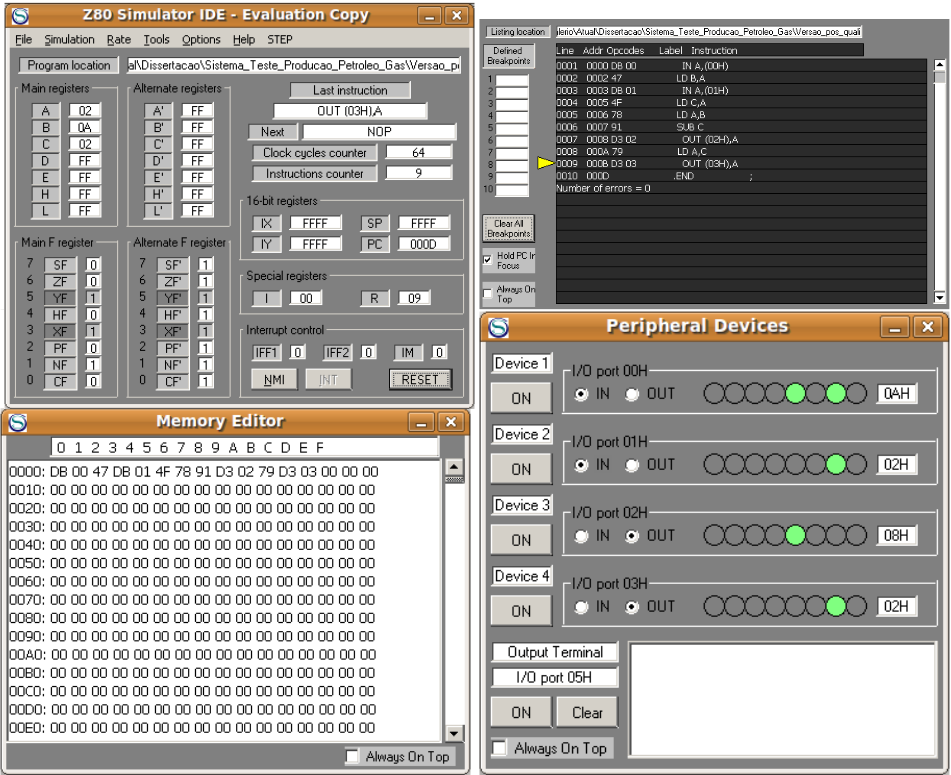
\includegraphics[width=1.0\textwidth]{images/Simulator_Full.png}
%\includegraphics[width=0.45\textwidth]{images/Simulator_Peripheral_Devices.png}
\caption{Window of Z80 simulator \cite{Simulator_z80}.}
\label{fig:simulacao}
\end{figure}



% Conclusão
\subsection{Final considerations }
%\subsection{Considerações finais sobre o estudo de caso}

%[Importáncia de ser o primeiro modelo 1° utilizando as bibliotecas]%[Completamente suportado pelo método B, principalmente devido ao uso de funções que convertem as representações dos sistemas de numeração]
%[A importáncia das técnicas e a experiência adquirida]
%[Explicar como pode ser útil para avaliar a vazão]
%[ Finalmente, argumento mais importante : A técnica está sendo viabilizada,
% pois o maior custo do processo está diminuindo devido aos avanços do atelierb e as técnicas descobertas  ]


The \textit{TestCalc\_basm} model was the first developed model according to
the proposal of \cite{Dantas_SBMF08} using the hardware and integer libraries. These
libraries contain type definitions, functions and lemmas that
could establish the relation between the B assembly model and its more
abstract model. These definitions kept the signature of operations relating to 
the B abstract model and the B assembly model; these simplified the
verification process and become more faithful to the representation of
microcontroller, everything without the need to extend the B method.

% % [Importáncia do 1° modelo]
% O modelo \textit{TestCalc\_basm} foi o primeiro construído de acordo com a proposta de [Dantas et al.
% 2008]  utilizando as bibliotecas de \textit{hardware} e tipos inteiros. Essas bibliotecas contêm tipos,
% funções e lemas que possibilitaram estabelecer a relação entre o modelo B \textit{assembly} e o modelo
% mais abstrato. Essas definições mantiveram a assinatura das operações do modelo abstrato com relação ao B
% \textit{assembly}, simplificaram o processo de verificação e tornaram mais fiel a representação do
% microcontrolador, tudo isso sem a necessidade de estender o método B.

The development of this model was too much important to improve the verification
process, because the development and verification help the design to get new
experiences with theorem prover (manual and interactive) and find proof
commands\footnote{The proof commands are steps that direct the prover to find the
proof, and cannot introduce false hypothesis.} that reduce too much the proof
process time. These experiences become the development and verification up to
assembly more feasible, mainly, because the most of the proof commands are
generic. So, these proof commands can be used again in several similar proof
obligations. In addition, the specification pattern used helps to model new and
different platforms.

% % [A importáncia das técnicas e a experiência adquirida]
% A elaboração desse modelo foi muito importante para amadurecer o processo de verificação, pois a
% construção e verificação do modelo ajudou ao projetista adquirir experiências com o provador interativo e
% a descobrir comandos de prova que reduzem significativamente o tempo do processo de prova. Essa
% experiência torna mais viável a especificação de outros \textit{softwares} mais complexos, pois a
% maioria dos comandos de provas podem ser usados novamente em obrigações de prova similares e o padrão de
% especificação utilizado ajuda na modelagem de novas plataformas. 

%No entanto, esse mesmo \textit{software} poderia ser acoplado em dispositivo \textit{timer} e 
%pois de forma bem eficiente foi resolvida  
%Certamente reduzem bastante o custo de verificação,
%pois o projetista desse modelo compreendeu a construção do invariante para linguagens assembly, 
%é possível aproveitar as caractéristicas das provas interativas para realizar algum tipo de automação nessa etapa,
%tudo indica que a construção da cláusula invariante pode ser feita por um algorítmo simples e    
%[Explicar como pode ser util para avaliar a vazão] ]
%Poderia se avaliando através da vazão, mas a modelagem ainda suporta bem aspectos temporais, por outro lado,
%utilizando-se de um dispotivo \textit{timer} esse mesmo \textit{software} poderia calcular o tempo de enchimento do tanque
%a vazão pode ser 

Finally, the developed embedded software can work like a redundant system and it
could provide a better confidence and quality, because the responsible engineer
has one more way to analyse the production test and more warranties. So, the
system can also improve the effectiveness of the test, because less failed tests
happen.

% %[ Importáncia para área de petróleo e gás ] Finalmente, o funcionamento do
% \textit{software} desenvolvido como um sistema redudante deve oferecer uma
% melhor confiança e qualidade, pois o engenheiro responsável terá mais um meio
% de comparação dos testes de produção e mais garantias. Essas garantias devem-se
% à existência de um sistema redundante e a sua verificação formal até um dos
% últimos níveis de representação do \textit{software}. Logo, o sistema pode
% também melhorar a eficácia dos testes, visto que menos testes falhos podem
% existir.






 
% \chapter{Projeto do compilador}
% \label{cap:proj_compilador}
% 
% % Intro
% Esta seção contém informações importantes sobre o projeto do compilador e
% ferramentas B, as quais podem ser reusadas nesse projeto. Adicionalmente, a atual
% seção apresenta duas abordagens possíveis para a construção do compilador. Desde
% já, é importante entender o contexto da relação entre o projeto do compilador e
% o estudo de caso.
% 
% 
% % Porque construir o compilador
% O estudo de caso descrito na seção \ref{sec:Bmodel_case_study} será refinado até o
% modelo algorítmico e posteriormente, o autor desse trabalho irá escrever
% manualmente o programa \textit{assembly} e o modelo B \textit{assembly}
% correspondente. No entanto, esse último passo pode ser automatizado através de um
% compilador específico. Por outro lado, o projeto desse tipo de compilador é uma
% atividade relativamente complexa, pois esse tipo de compilador deve também
% introduzir fórmulas no modelo B \textit{assembly} para possibilitar o processo
% de verificação, de acordo com o que foi explicado no capítulo
% \ref{cap:VerificacaoAssembly}.
% 
% Dessa forma, o presente trabalho fornecerá apenas informações úteis para o seu projeto inicial.
% 
% \subsection{Reuso do \textit{parser}}
% % Explicar que é possível reusar o parser
% Para a construção do compilador é possível reusar o
% \textit{parser}\footnote{\textit{Parser} é um componente de \textit{software} que
% reconhece uma sequência de caracteres de entrada (código fonte) e constrói uma
% estrutura de dados para representação e manipulação dessa entrada.} de uma outra
% ferramenta. Na comunidade existem vários \textit{parsers} para método B, no
% entanto será comparado apenas os quatro mais significativos e viáveis. Esses
% \textit{parsers} são utilizados nas seguintes ferramentas:
% \textit{ABTools}, \textit{BSmart/Batcave},  \textit{BParser} e \textit{ComenC}.
% 
% O \textit{ABTools} segundo \cite{DBLP:conf/acsd/Boulanger03} é um ambiente de
% desenvolvimento B composto de \textit{parser}, verificador de tipos, gerador:
% de obrigações de prova e documentação. \textit{ABTools} foi desenvolvido com o
% intuito de facilitar o desenvolvimento de ferramentas de extensão para linguagem
% B, o que é interessante para o projeto do compilador com verificação em nível de
% \textit{assembly}. Por outro lado, o \textit{ABTools} não vem sendo muito
% utilizado na indústria, o que não demonstra um forte amadurecimento.
% 
%  
% As ferramentas \textit{BSmart}~\cite{deharbe06developing} e
% \textit{Batcave}\\\cite{Batcave} utilizam um único \textit{parser}, esse
% \textit{parser} é uma evolução do utilizado na ferramenta
% \textit{JBTools}~\cite{Tatibouet}. O \textit{parser} é desenvolvido na linguagem
% \textit{Java}~\cite{Java} e utiliza o gerador de \textit{parser}
% Javacc~\cite{Javacc}. \textit{Java} e \textit{Javacc} são bastante conhecidos na
% comunidade e possuem ampla documentação disponível, o que facilita o
% desenvolvimento do compilador. Por outro lado, segundo~\cite{Fabian2008}, o
% \textit{parser} do \textit{JBTools} usa uma árvore sintática com elementos
% desnecessários e ele é difícil de manter e estender. Os empecilhos citados
% levaram à construção de um novo \textit{parser}, chamado \textit{BParser}.
% 
% O \textit{BParser}~\cite{Fabian2008} (\textit{Object Oriented Parser For B Specifications}) foi construído para ser
% utilizado pelo \textit{ProB}~\cite{proB} e tinha como principais objetivos: melhorar a capacidade de manutenção e
% extensão, e suportar completamente a sintaxe de B. Além disso, o \textit{BParser} tem código fonte cinco vezes
% menor que \textit{parser} do \textit{JBTools}. Entretanto, o \textit{BParser} apresentou pequenos problemas em testes
% realizados pelo autor desta dissertação, mas eles foram corrigidos rapidamente pelo autor do \textit{BParser}.
% Logo, isso indica que o \textit{BParser} está em fase de amadurecimento. Outro \textit{parser} mais estável e
% utilizado em escala industrial é o embutido na ferramenta \textit{ComenC}~\cite{ComenC}.
% 
% O \textit{ComenC} é um tradutor de B para a linguagem C. Ele é resultado da convergência de trabalhos
% entre a indústria e a pesquisa. Dessa forma, o \textit{ComenC} tem uma versão de \textit{software} bem estável e
% recentemente vem disponibilizando atualizações com frequência. Adicionalmente, existe uma ampla documentação
% disponível sobre o \textit{parser} do \textit{CommenC} e ele segue as especificações padrões da
% linguagem B utilizada na indústria. Portanto, o \textit{parser} do \textit{ComenC} é um forte candidato a ser
% utilizado no projeto do compilador.
% 
% 
% A Tabela \ref{tab:Comparacao_parsers} contém uma síntese comparativa com as principais características das
% ferramentas, as quais podem ter o \textit{parser} reusados.
% 
% \begin{table}[h]
% \begin{center}
% \begin{tabular}{|l|c|c|c|c|c|c|}
% \hline
%   & \textbf{ABTools}  & \textbf{BSmart/Batcave}  &  \textbf{BParser} &  \textbf{ComenC}  \\
%    \hline
%  Idioma & Francês/Inglês & Português/Inglês  &  Inglês/Alemão &  Francês/Inglês  \\
%  \hline
%  Tecnologias & ANTLR & Java/Javacc  &   Java/SableCC & C++/C \\ \hline
%  Código aberto &  Sim &  Sim  &  Sim  & Sim \\ \hline
%  Licença &  \textit{GNU LGPL} &  \textit{GNU LGPL} & Não
%  definido &  \textit{GNU GPL}\\ \hline
%  %Mês da última versão & 08/2008  & 02/2008 & 05/2009  \\ \hline
%  Apoio & INRETS &  UFRN  & Heinrich-Heine & Clearsy  \\ \hline
% \end{tabular}
% \end{center}
% \caption{Tabela comparativa com características das ferramentas para o método B.}
% \label{tab:Comparacao_parsers} 
% \end{table}
% 
% 
% \subsection{Abordagens para construção do compilador}
% \label{sec:proj_compilador}
% 
% 
% A princípio, existem duas abordagens possíveis para a construção do compilador. Essas abordagens são
% ilustradas através de dois diagramas de comunicação da UML, que mostram as colaborações após a verificação do
% modelo algorítmico.
% 
% A abordagem mais simples é ilustrada no diagrama de comunicação da Figura~\ref{fig:poucoreuso}. Nessa abordagem é
% construído um único novo componente de \textit{software}, que aproveita um \textit{parser} desenvolvido anteriormente e
% adiciona a funcionalidade de transformar o modelo algorítmico B em \textit{assembly} e B \textit{assembly}. Então, o
% próprio AtelierB deve verificar a consistência do código gerado. Logo, essa abordagem é simples, pois o
% desenvolvedor provavelmente deve trabalhar com apenas uma tecnologia e componente de \textit{software}.  
% 
% 
% \begin{figure}[h]
% \centering 
% \includegraphics[width=0.85\textwidth]{images/Diagrama_Comunicacao_Simplificado.png}
% \caption{Diagrama de comunicação do processo de compilação e verificação na abordagem simplificada.}
% \label{fig:poucoreuso}
% \end{figure}
% 
% % Como funciona ?
% Uma segunda abordagem para o projeto do compilador é ilustrada na
% Figura~\ref{fig:altoreuso}. Essa abordagem separa as responsabilidades em vários
% componentes de \textit{software}. Além disso, ela intensifica ainda mais o reuso.
% Após os passos do método B tradicional, a segunda abordagem funciona da seguinte
% forma: inicialmente é utilizado o \textit{ComenC} para gerar código C; na
% sequência é utilizado o popular compilador \textit{gcc}~\cite{gcc}, ou qualquer
% outro compilador C, para gerar código assembly para o Z80; após isso, o módulo de
% \textit{software} ASM2BASM, a ser desenvolvido, deve transformar código \textit{assembly} puro para
% B \textit{assembly}; finalmente, o \textit{AtelierB} deve verificar se o código é
% consistente com relação ao modelo refinado. Essa abordagem não é muito
% recomendada para o desenvolvimento com uma equipe pequena, pois um grande esforço
% será necessário para compreender detalhes de todos os componentes de
% \textit{software} envolvidos. Adicionalmente, essa abordagem possivelmente
% dificultará a geração dos invariantes e variantes do modelo \textit{assembly}.
%  
% 
% \begin{figure}[h]
% \centering 
% \includegraphics[width=0.999\textwidth]{images/Diagrama_comunicacao_com_muito_Reuso.png}
% \caption{Diagrama de comunicação do processo de compilação e verificação na abordagem com alto reuso.}
% \label{fig:altoreuso}
% \end{figure}
% 
% %Resumo da comparação das duas abordagens
% 
% A grande vantagem da abordagem mais simples é a exigência de uma equipe menor de trabalho. Além disso, resultados
% iniciais podem ser obtidos mais rapidamente. Por outro lado, a segunda abordagem é mais audaciosa, generalista e
% pode aproveitar a capacidade do \textit{gcc} de gerar código \textit{assembly} para várias plataformas.
%  
% Finalmente, o projeto do compilador deve evoluir de acordo com as experiências obtidas nesse estudo de caso real.
% Desta forma, as dificuldades e as novas soluções encontradas colaborarão diretamente para construção do compilador.
% 
%    
% \subsection{Plano de desenvolvimento dos trabalhos propostos}
% \label{sec:cronograma}
% 
% As atividades discentes planejadas para o segundo semestre deste ano estão relacionadas com: a modelagem e
% verificação do estudo de caso da seção \ref{sec:Bmodel_case_study}; relato de informações úteis ao projeto do compilador;
% e a elaboração da dissertação.
% 
% \begin{enumerate}
% 
% \item A modelagem e a verificação do estudo de caso são realizadas em 4 etapas:
% 	\begin{enumerate}
%       \item A construção e verificação do modelo funcional;
% 	  \item A elaboração e verificação do seu refinamento e modelo algorítmico;
% 	  \item A implementação do código \textit{assembly} correspondente;
% 	  \item A construção e verificação do modelo B \textit{assembly}. Essa última
% atividade é uma das etapas mais complexas e difíceis, no entanto, tal atividade é a mais importante para
% o objetivo desse trabalho.
% \end{enumerate}
% 
% % Inicialmente, os trabalhos serão realizados sobre um subconjunto da linguagem
% % de B. Nesse sentido, uma gramática BNF foi desenvolvida e está nos anexos desse
% % trabalho (capítulo \ref{cap:anexo}).
% \item Quanto ao projeto do compilador citado anteriormente, informações na
% dissertação serão apenas descritas,  se eventualmente essas forem úteis para o
% compilador.
%  
% \item Com relação à dissertação, a escrita será realizada, aos poucos, com o
% decorrer do desenvolvimento da modelagem e verificação do estudo de caso. Os
% capítulos \ref{cap:MetodoB},\ref{cap:VerificacaoAssembly} e
% \ref{cap:trabalhosdesenvolvidos} deste trabalho estão praticamente prontos para
% dissertação. Então, falta apenas relatar sobre a modelagem do estudo de caso e
% realizar alguns ajustes na introdução e conclusões. Finalmente, pouco tempo antes
% da defesa será intensificada a escrita da dissertação.
% 
% \item Para a defesa será elaborada a apresentação e a revisão os últimos detalhes do trabalho. 
% 
% \end{enumerate}
% % Elaboração de estudo de caso - Estudar em mais detalhes o estudo de caso.
% % 							 - Construir um modelo funcional e validar o modelo.
% % 							 - Elaborar os demais modelos algoritmos
% % 							 
% % Compilador 					 - Será relatado alguma ideia, caso surja.
% % 							 -  
% %  
% % Dissertação					 - Ir elaborando paralelamente de acordo com o desenvolvimento dos trabalhos.
% %\newpage
% 
% % O cronograma para realização dessas atividades discentes é apresentado na Tabela~\ref{cronograma}.
% % 
% % \newcommand{\drawbox}{\rule[0mm]{10mm}{3mm}}
% % \begin{table}[!h]
% % \begin{center}
% % \begin{small}
% % \begin{tabular}{|c|c|c|c|c|c|}
% % \hline  & {\bf Jul.} & {\bf Ago.}  & {\bf Out.} & {\bf Nov.}  & {\bf Dez.}\\
% % \hline
% % 1(a)   & \drawbox  &   &   &   &   \\
% % 1(b)   & \drawbox  &  \drawbox  &  &   &   \\
% % 1(c)   & \drawbox &   \drawbox &   &   &   \\
% % 1(d)   & \drawbox  & \drawbox  & \drawbox  &   &   \\
% % 2   &   & \drawbox  & \drawbox  & \drawbox  &   \\
% % % 2(c)   &   &   &   &   & \drawbox  \\
% % % 3(a)   &   &  \drawbox & \drawbox  & \drawbox  & \drawbox  \\
% % % 3(b)   &   &  \drawbox & \drawbox  & \drawbox  & \drawbox  \\
% % % 3(c)   &   &   &   &   &   \\
% % 3   & \drawbox  & \drawbox  & \drawbox  & \drawbox  & \drawbox  \\
% % 4   &   &  &   &   & \drawbox  \\  
% % \hline
% % \end{tabular}
% % \end{small}
% % \end{center}
% % \caption{Cronograma para o desenvolvimento das atividades discentes}
% % \label{cronograma}
% % \end{table}
% % 
% 

\section{Verification Process}
\label{sec:Verification}

% [O que as provas garantem? citar que dificeis, que he necessherio buscar thecnicas eficientes
% para realizar as provas ]
This section describes the verification process of B model of instructions set
and B model in assembly-level. The proof obligations allow to verify the data
types, important system properties and if the expressions are well-defined (WD). The
properties provide additional guarantees, because they can set many
safety rules. However, the model can be very difficult to prove without using
different strategies.


The use of proof commands can accelerate the verification process, therefore two
proof commands are simple, effective, efficient and useful; they are presented
in~\ref{subsection:VerificationInstructions}. When these two commands are used is
recommended to set the time out of theorem prover to one second, which is enough
to solve the vast majority of proof obligations and prevent the theorem prover
waste time unnecessarily in proof obligations that are not resolved by these
proof commands. The next two subsections present these two proof commands that
solve quickly the most of proof obligations.

% O uso de comandos de prova pode acelerar bastante o processo de prova, portanto
% dois comandos de provas simples,  eficazes, eficientes e muito úteis são
% apresentados. Quando esses dois comandos de provas são utilizados é recomendado
% ajustar o \textit{time out} do provador para 1 segundo, o que é suficiente para
% resolver a grande maioria das obrigações de prova e isso evita que o provador
% desperdice muito tempo desnecessariamente em obrigações de prova que não são
% resolvidas por estes comandos.



The verification process is organized in groups two groups: instructions set
verification and assembly-level verification.

\subsection{Verification process of instructions set model} 
\label{subsection:VerificationInstructions}
The following proof command is used to solve the most of WD proof obligatios of
Z80 model. This proof command is applied in proof obligations that satisfy the pattern: $x \in dom(y)$.
The sequence of commands: select the minimum force in theorem prover, remove the obvious hypothesis from stack, 
replace the term $dom(y)$ for an equivalent expression, execute the simplifier
and the automatic prover.

% O comando de prova seguinte é utilizado para resolver a maioria das obrigações de prova EBD do modelo do
% Z80. Esse comando de prova é aplicado nas obrigações de prova que satisfazem o padrão: $x \in dom(y)$.
% A sequência de comandos: seleciona a força mínima do provador, remove as hipóteses óbvias da pilha,
% substitui o termo $dom(y)$ por um equivalente, executa o simplificador e o provador automático.

\begin{center}
\framebox(350,70)[c]{ Pattern( x $\in$ dom(y) ) \& ff(0) \& dd \& eh(dom(y)) \& ss \& pr }
\end{center}


Some statistics proofs of instructions set model are shown below:
%[Groups]
\begin{center}
\begin{tabular}{llll}
\textbf{Instructions Groups} &  \textbf{Proofs No Obvious} & \textbf{Proofs WD}
& \\ Input and Output & 54 & 296  \\ 
Logic and Arithmetic & 134 & 413  \\ 
Manipulation of Bits & 160 & 742  \\ 
Extern actions & 51 & 84  \\
General & 140 & 615  \\
Initialization, Properties and Assertions & 68 & 169  \\
 \textbf{Total} &  607 &  2319  &  %\textbf{Total} 2926 \\
\end{tabular}
\end{center}


% [Conclusao] This project has many proof obligations and
% The construction of then model was a difficult task, as several
% iterations were needed to provide the good library definitions
% as well as to optimize the definition of the functionality of
% the microprocessor instructions by grouping common data
% manipulation into auxiliary functions.

Several iterations were needed to provide the good library definitions as well as
to fine-tune the model of the microcontroller instructions by factoring common
features into auxiliary definitions.


However, few proof commands need to be used to prove most proof obligations. As
there are many similar assembly instructions, some human-directed proofs, when
replayed, could discharge other proof obligations. A good example is a set of 17
proof commands that quickly aided the verification of 99\% (2295) of WD proofs.
We also set up a proving environment consisting of networked computers to take
advantage of the distribution facilities now provided in the B development
environment. Finally, all of the 2926 proof obligations were proved using the
tool support of the development environment.


\subsection{Verification process of B assembly model }
% /Processo de verificação do modelo B assembly}

% O modelo \textit{TestCalc\_basm} continha 200 obrigações de prova
% do tipo EBD (Expressões Bem Definidas) e 568 não óbvias. As obrigações de prova EBD foram rapidamente
% resolvidas através de comandos de prova e do provador interativo. As outras 568 não foram resolvidas tão
% facilmente. Felizmente, existe um comando de prova extremamente eficiente que agiliza a verificação, pois
% esse comando de prova é reusável em obrigações de prova semelhantes, as quais são comuns na modelagem B
% \textit{assembly}.

The model \textit{TestCalc\_basm} has 200 WD proof obligations and 568 no obvious
proof obligations. The well defined proof obligations were verified quickly
through proof commands and the interactive prover. The others 568 were not solver
as quickly. Fortunately, there is an extremely efficient proof command, because
this proof command is reusable and fast to solve other similar proof
obligations, which are often in B assembly modelling.


%O comando de prova definido a seguir foi utilizado para resolver 81\% das obrigações de prova do modelo
%\textit{TestCal\_basm}. A sequência de comandos: seleciona a força mínima do provador e executa o provador
%tático com o conjunto de regras \textit{ContradictionXY}.

The following defined proof command was used to solve 81\% of proof
obligations of \textit{TestCal\_basm} model. The sequence of commands: select the minimum force of prover and execute the
automatic theorem prover using the contradiction tactic.

\begin{center}
\framebox(220,70)[c]{ ff(0) \& pr(Tac(ContradictionXY)) }
\end{center}

% Este comando de prova praticamente resolve todas as obrigações de prova as
% quais representam um fluxo de execução inválido, isto é, no caso do modelo
% \textit{TestCalc\_basm} representam a possibilidade de fluxos de execução não
% lineares. Essas obrigações de prova são criadas porque o gerador de obrigações
% de prova constrói fórmulas para avaliar todas as posibilidades do fluxo de
% execução do modelo. Como o modelo especificado tem um fluxo de execução linear,
% ou seja, o contador de programa ($\mathit{pc}$) efetua apenas saltos para a
% instrução seguinte, então o número de possibilidades do fluxo de execução é
% mínimo. 
% Nesse caso, o comando de prova citado ajudou a verificar rapidamente
% 465 obrigações de prova (81\%). Um fato ainda mais interessante é que foi
% utilizado um \textit{time out} de um segundo para resolver cada obrigação de
% prova. Dessa forma, foi necessário no máximo 465 segundos para resolver 81\%
% das obrigações de prova. As 103 demais obrigações de prova foram resolvidas
% interativamente, pois essas eram mais complexas\footnote{Nenhuma das 103
% obrigações de prova foi resolvida no provador automático na força zero e com um
% \textit{time out} de 180 segundos.}. Para esse comando de prova funcionar é
% importante declarar no invariante do \textit{while} de cada instrução os
% possíveis próximos valores do contador de programa. Esse e outros comandos de
% prova podem ser consultados no anexo deste trabalho.

This proof command solves almost all proof obligations that represent a no
linear execution flow. These proof obligations are created because the proof
obligation generator builds formulas to verify every possible execution flow.
The specified model has a linear execution flow, in others words, the program counter
($\mathit{pc}$) does only jump forward, then the possibility number of execution
flow is few. In this model, the proof command quoted helps to verify quickly
465 proof obligations (81\%). A fact more interesting is the time out used, with
this proof command, that is just one second. Thus, in the maximum 465 seconds,
81\% proof obligations were solved. The others 103 proof obligations were solved
using the interactive prover, because the proof obligations were more
complex\footnote{Neither of 103 proof obligations were solved using the
automatic prover with force zero and time out equal 180 seconds}.



% Nesse modelo os passos das provas interativas seguem alguns padrões, os quais foram identificados pelo projetista
% e isso ajudou bastante a verificação. Contudo, o projetista ainda não conseguiu definir uma sequência de comandos de prova 
% suficientemente genérica para resolver várias obrigações de prova entre as 103 não resolvidas
% automaticamente. Finalmente, a construção de um invariante válido e a realização das provas interativas
% do modelo \textit{TestCal\_basm} apresentado anteriormente são as atividades mais complexas do processo
% de verificação, já que essas duas atividades consomem aproximadamente 70\% e 80\% de todo o processo de especificação e
%  verificação.

The steps used in interactive prove follow patterns, that were identified during
design stage and it helps too much the verification. However, the designer needed
to verify 103 proof obligations almost manually, using the interactive prover.
Finally, the construction of a valid invariant and the verification of manual
proofs of \textit{TestCal\_basm} presented before are the activities more complex
of verification process, because these activities spend approximately 75\% of
time of specification and verification process.






\subsection{Final considerations about verification process}

The level of automation of proof process was satisfactory, because the B method,
its tools and features were too much explored. Case the proof process have gotten
a low automation then the proof process could be very slow and difficult. Two
requirements are important to verify quickly the proof obligations: a experience
with interactive theorem prover from Atelierb~\cite{CLEARSY}, that is acquired
from practicing, and knowledge about proof commands (mathematical
rules)\cite{ClearsyMathRule}.

Naturally, the statics confirms the good level of proof process automation: in B
instruction set models approximately 89\% of obvious proof obligations and 99\%
proof obligations well defined were verified automatically; and in B assembly
model 465 of obvious proof obligations were verified automatically. A design with
good division responsibility of modules reduces efforts. The modularization helps
to build two simple libraries that defines important basic lemmas, and also
separated and organized the instructions specification in different modules, it
was important to verify the models in parallel.

To verify the proof obligations from different modules were used four computers,
each one with two cores. The parallelization of proof process also increases many
times the processing capacity. So, the set of techiques used in verification
process was essential to accelerate verification process.

\section{Related works}
\label{sec:relatedworks}
 
There are in the literature of computer science some
approaches~\cite{BHDL_2003,GEMPLUS_99,DBLP:journals/entcs/EvansG08,DBLP:conf/fmco/Leuschel08,DBLP:conf/asm/Wright08}
to model hardware and the virtual machines using B. Then, in these works the B
method has been used successfully to model the operational semantic. However the
cost of modelling was still expensive and this report quoted some techniques to
lower the cost of modelling.
% Although, the modelling of the Z80 do not have modelled some small aspects.


% The objective of researchers


In general, the researchers employing the B method have focused on
more abstract level of description of software.  Considering low-level
aspect, there has been previous work on modelling the Java Virtual
Machine~\cite{GEMPLUS_99}.

The main motivation of our research is the development of verified
software up to the assembly level, which requires specifying the
semantics of the underlying hardware. Thus some aspects were not
modelled in our work such as the execution time of the instructions.
Also we did not consider the micro architecture of the hardware as the scope of
our work does not include hardware verification. However, there are
many other specialized techniques to verify these questions.
 
\section{Conclusions}
\label{sec:conclusions} 
[I need do english review]\\
% Um pequeno resumo do trabalho
This work has shown an approach to the formal modelling of the instruction set of
microcontroller using the B method. During the construction of this model, some
problems were found in the official reference for Z80
microcontroller~\cite{Z80_manual}. The designer fixed the found problems in
documentation and also developed a case study: a verified embedded software. This
case study was interesting to analyse the techinque of formal verification up to
assembly level. 
% ____________
% % motivação continuação do resumo do trabalho
% The focus of this researh is related with the consistency of generated assembly
% code after the use of traditional B method. So, it is not in scope of more
% important B tools\cite{CLEARSY,DBLP:conf/tapsoft/B-Core95,proB}. The
% introduction of errors in assembly code is rare. But it is very difficult to
% identify, mainly, because the software debugging in assembly language is very
% complex. 
% 
% % Motivação para o trabalho > sem muito foco \ldots
%  O problema principal desta pesquisa é relativo com
% consistência do código assembly gerado após a aplicação do método B, o que
% não está no escopo das mais importantes ferramentas de suporte B [Clearsy
% 2009, B-Core 1995, Leuschel e Butler 2003]. A introdução de erros no código
% assembly é um acontecimento raro e de difícil diagnóstico, principalmente
% porque a depuração de software na linguagem assembly é muito complexa.
% Um fato mais comum que pode provocar a mudança da semântica do software é
% quando acontece a alteração do compilador ou da versão do compilador.
% Portanto, esse tipo de mudança é um forte ponto de risco.
% 
% Um cuidado especial deve ser tomado com o processo de transformação de código
% para a linguagem assembly, principalmente nos compiladores utilizados em menor
% escala, os quais normalmente possuem um escopo de teste de utilização menor
% que os compiladores tradicionais\cite{gcc}. Este é exatamente o caso do
% compilador do Z80.
% 
% -> Uma proposta para solução desses problemas é apresentada nesse trabalho.
% 
% 
% % Caractéristicas positivas da metodologia \ldots 
% 
% % Fechamento do trabalho com Chave de ouro
% %Util para o fechamento com chave de ouro
% Os resultado deste trabalho são muito importantes \ldots
% 
% As the B notation has a syntax that is not too
% distant from that of imperative programming languages, such model could be used
% to improve the documentation used by assembler programmers. Besides, the formal
% notation used is analysed by software that guarantees the correctness of typing,
% the well-definedness of expressions, in addition to safety properties of the
% microcontroller state.
% 
% % mostra as utilidade do trabalho para modelar hardware.
% Os resultados desse trabalho demonstram a viabilidade da proposta de
% desenvolvimento formal até o nível de assembly, pelo menos para sistemas de
% pequeno porte. Esses resultados mostram também que as linguagens de
% especificações formais para software podem ser usadas para de􏰅nir a semântica
% do conjunto de instruções de microcontroladores e microprocessadores.
% 
% 
% ------------
Some activities were very useful to accelerate the used
metodology: development of hardware library and types library, parallezation of
proof process, construction of generic proof commands and many hours working
with on interactive prover. Theses activities resulted some works.


% Os meus trabalhos já desenvolvidos/ resultados atuais.
The first work \cite{DantasSemish2008} shows the developed metodology to verify
software up to assembly level using B. A second work\cite{Dantas_SBMF08}
presents more details about the verification approuch and a small example
software verified up to assembly level in three differents plataforms. 
The work \cite{Ermac2008} describe the developed librarys and a Z80 initial
model. The last work \cite{SBMF2009_micro} shows a general view of the full Z80
model and tecniques used in verification proccess.

%Link com o parágrafo anterior 
These quoted works do a important step to software verification up to assembly
language, they show the actuals difficulties and suggest improvements in the
B tools. 





% [Trabalhos futuros ] LLVM:Existe também a pretensão de especificar as

Future works comprise the development of software with the B method from
functional specification to assembly level, using the Z80 model presented in this
work. The mechanic compilation from B algorithmic constructs to assembly platform
is also envisioned. Finally, another important activity is adjust the
specification to be able animate in ProB\cite{proB} the B assembly specification
and the Z80 model.



  
%\paragraph{Acknowledges:}
%This work was partially supported by INES (www.ines.org.br), funded by CNPq
%grant \ldots
%573964/2008-4 and by CNPq grants 553597/2008-6, 550946/2007-1, and 620132/2008-6..

\bibliographystyle{splncs}
\bibliography{paper}
% [To change the format; to add: thesis suggested by David, Article from ABZ 2010 suggested by David  ]
% \begin{thebibliography}{5}
% 


\end{document}
%
% \bibitem {clar:eke}
% Clarke, F., Ekeland, I.:
% Nonlinear oscillations and
% boundary-value problems for Hamiltonian systems.
% Arch. Rat. Mech. Anal. {\bf 78} (1982) 315--333
% %
% \bibitem {clar:eke:2}
% Clarke, F., Ekeland, I.:
% Solutions p\'{e}riodiques, du
% p\'{e}riode donn\'{e}e, des \'{e}quations hamiltoniennes.
% Note CRAS Paris {\bf 287} (1978) 1013--1015
% %
% \bibitem {mich:tar}
% Michalek, R., Tarantello, G.:
% Subharmonic solutions with prescribed minimal
% period for nonautonomous Hamiltonian systems.
% J. Diff. Eq. {\bf 72} (1988) 28--55
% %
% \bibitem {tar}
% Tarantello, G.:
% Subharmonic solutions for Hamiltonian
% systems via a $\bbbz_{p}$ pseudoindex theory.
% Annali di Matematica Pura (to appear)
% %
% \bibitem {rab}
% Rabinowitz, P.:
% On subharmonic solutions of a Hamiltonian system.
% Comm. Pure Appl. Math. {\bf 33} (1980) 609--633
% \end{thebibliography}
%

